%%%%%%%%%%%%%%%%%%%%%%%%%%%%%%%%%%%%%%%%%%%%%%%%%%%%%%%%%%%%%%%%%%%%%%%%%%%%%%
%  IEEE Transactions-style paper (IEEEtran, journal option)
%  A PUF-Based Four-Phase Authentication Framework for UAV Swarms
%%%%%%%%%%%%%%%%%%%%%%%%%%%%%%%%%%%%%%%%%%%%%%%%%%%%%%%%%%%%%%%%%%%%%%%%%%%%%%
\documentclass[journal]{IEEEtran}
\IEEEoverridecommandlockouts

\usepackage{cite}
\usepackage{amsmath,amssymb,amsfonts}
\usepackage{amsthm}
\usepackage{bm}
\usepackage{algorithmic}
\usepackage{graphicx}
\usepackage{textcomp}
\usepackage{xcolor}
\usepackage{booktabs}
\usepackage{multirow}
\usepackage{array}
\usepackage{url}
\usepackage{float}
\usepackage{tikz}
\usetikzlibrary{arrows.meta,positioning,calc,patterns}
\usepackage{pgfplots}
\pgfplotsset{compat=1.18}

\newtheorem{theorem}{Theorem}
\newtheorem{lemma}[theorem]{Lemma}
\newtheorem{corollary}[theorem]{Corollary}
\newtheorem{definition}{Definition}

\begin{document}

\title{A PUF-Based Four-Phase Authentication Framework for UAV Swarms: Design,
Provable Security, and a Measured OMNeT++ Evaluation}

\author{Md~Ziyad~Hussain,~\IEEEmembership{Student Member,~IEEE,}
        and~Rakesh~Matam,~\IEEEmembership{Member,~IEEE}%
\thanks{Md Ziyad Hussain and Rakesh Matam are with the Department of Computer
Science and Engineering, Indian Institute of Information Technology Guwahati,
Bongora, Assam 781015, India (e-mail: ziyad.hussain23b@iiitg.ac.in;
rakesh@iiitg.ac.in).}%
\thanks{This work was carried out under the guidance of Dr.\ Rakesh Matam at
IIIT Guwahati.}}

\markboth{IEEE Transactions on Dependable and Secure Computing}%
{Hussain \MakeLowercase{\textit{et al.}}: A PUF-Based Four-Phase Authentication Framework for UAV Swarms}

\maketitle

\begin{abstract}
UAV swarms need authentication that is fast, light, and survives the physical
capture of individual drones. Conventional mechanisms fail somewhere on that
list: RSA and ECC handshakes keep a private key in non-volatile memory, and
pre-shared keys collapse swarm-wide when one node is taken. We present a
four-phase authentication framework whose root of trust is a Physical
Unclonable Function (PUF), so the key is the silicon itself and nothing secret
is ever stored. Phase~1 performs one-time enrollment in a secure facility and
turns noisy PUF measurements into a stable per-device master key through a
code-offset fuzzy extractor over BCH(255,131,18), publishing only helper data.
Phase~2 is a four-message mutual-authentication handshake between a UAV and its
Ground Station (GS) in which every message carries a keyed MAC, the raw PUF
response never leaves the device, and the drone refuses to answer until it has
verified the GS. The handshake also delivers per-pair credentials under
authenticated encryption, so Phase~3 lets any two drones authenticate each
other with no GS round trip while a captured drone exposes only its own links.
Phase~4 folds a mandatory authenticated ephemeral Diffie--Hellman secret into
every session key, giving perfect forward secrecy. We prove six security
properties, mutual authentication in both directions, peer authentication,
replay and man-in-the-middle resistance, session-key secrecy with forward
secrecy, and capture boundedness, each reduced to standard assumptions, and
corroborate them with a Tamarin symbolic model. A reference implementation
comprises 8{,}585 lines of C++17 on OMNeT++~6.3 plus 4{,}125 lines of tests,
with two interchangeable crypto suites (SHA3-based and SPONGENT-based), three
PUF models, and three fuzzy-extractor profiles, and every primitive is checked
against published vectors where they exist. Sixteen configurations, thirty
repetitions each, were executed on one host: all 600 UAVs and all 11{,}400
peer-pair views of a twenty-drone swarm authenticate, at $0.57 \pm 0.04$~ms of
compute and $1.07$~ms of modelled network delay per UAV--GS handshake and
$0.4167 \pm 0.0006$~ms per peer pair. The fuzzy extractor's measured failure
rate tracks its binomial
prediction across four orders of magnitude. Executed attacks, including a
negative-control ablation, reproduce the analysis. Measured against real
RSA-2048 and ECDSA-P256 handshakes on the same simulator, the framework costs
$1.64$~ms against $1.77$~ms and $0.79$~ms respectively, and over a real
IEEE~802.11 stack end-to-end latency reaches $7.9\times$ the idealised medium
while the framework's own compute is unchanged, so the increase is the channel
rather than the protocol. The advantage of the framework is
therefore argued as a set of properties, no stored long-term secret, no
certificate infrastructure, GS-free peer authentication, and bounded capture
damage, rather than as raw speed, and the costs are reported as measured.
\end{abstract}

\begin{IEEEkeywords}
UAV swarm, physical unclonable function, PUF, fuzzy extractor, BCH code,
mutual authentication, forward secrecy, lightweight cryptography, SPONGENT,
OMNeT++.
\end{IEEEkeywords}

%=============================================================================
\section{Introduction}
\label{sec:intro}
%=============================================================================

Unmanned Aerial Vehicles now operate as coordinated swarms: ten to twenty
drones covering a stadium, a border strip, or a disaster zone, continuously
linked to a Ground Station (GS) on a command-and-control channel and to one
another on peer links for formation control and sensor fusion~\cite{securing_uav_fanet}.
Before any of that traffic can be trusted, each drone must verify the identity
of its GS and of every peer, and each side must prove itself. Without it, an
adversary can inject a rogue drone into the formation, read the telemetry, or
issue flight commands~\cite{puf_uav_cross_domain}.

The classical mechanisms fit this regime poorly, and for one recurring reason.
\textbf{RSA-2048} costs about a millisecond per signature on hardware a drone
can actually carry, and attaches hundreds of bytes of certificate to every
handshake~\cite{puf_lightweight_uav}. \textbf{ECC-256} is much cheaper but still
keeps a private key in non-volatile memory (NVM) that a captured drone can
surrender through a cold-boot or side-channel attack~\cite{peer2peer_auth}.
\textbf{Pre-shared keys} are sub-millisecond and then compromise the entire
swarm the moment any single device is captured, and they scale as $O(N^2)$
pairwise keys~\cite{puf_iot_strong_adversary}. \textbf{Blockchain-based}
schemes incur seconds of consensus latency that real-time formation control
cannot absorb~\cite{puf_ntu}. A common thread runs through all of them: a
long-term secret \emph{stored} on a device that can physically fall into an
adversary's hands.

A Physical Unclonable Function (PUF) removes that secret. It maps challenges to
responses using sub-nanometre manufacturing variation that is unique to one
integrated circuit: two nominally identical chips answer the same challenge
with about 50\% Hamming distance between responses, one chip answers its own
challenge with a few percent of drift, nobody, including the manufacturer, can
reproduce the mapping, and invasive probing destroys it~\cite{puf_overview}. An
Arbiter PUF needs roughly 1{,}200 gate equivalents. The key is the silicon, so
there is nothing in memory to steal. The catch is noise: a raw PUF response is
a fingerprint, not a key, until a fuzzy extractor reconciles it.

\subsection{Design goals and threat model}

The framework targets nine properties: (1) mutual authentication in both
directions, checked by keyed MACs; (2) anonymity through rotating temporary
identities; (3) replay and man-in-the-middle resistance through nonces,
timestamps, and transcript binding; (4) \emph{no stored secret} on the drone,
with the master key regenerated from the PUF on demand; (5) GS-free peer
authentication rooted in per-pair credentials; (6) perfect forward secrecy
through a mandatory ephemeral key exchange; (7) light operation, one hash, a
keyed MAC, an AEAD, a KDF, and one elliptic curve; (8) scalability, since the
$O(N^2)$ peer exchanges are independent and parallel; and (9) noise tolerance
through the BCH fuzzy extractor.

The threat model is a Dolev--Yao adversary~\cite{dolev_yao} with physical reach.
It may eavesdrop, intercept, modify, replay, delay, or drop any wireless
message; it may pose as the GS toward an honest drone and send adversarially
chosen challenges and nonces; it may seize drones and read their NVM, but it
cannot clone PUF hardware, since invasive probing destroys the response; it is
bounded to probabilistic polynomial time, so it cannot invert the hash, forge a
MAC or an authenticated ciphertext, break PUF unpredictability, or solve
computational Diffie--Hellman except with negligible probability; and standard
side-channel countermeasures are assumed on the devices.

\subsection{Contributions}

\begin{enumerate}
\item \textbf{A stable PUF-derived key with no stored secret.} Enrollment
distils a per-device master key through a fuzzy extractor; the drone
regenerates it on demand from its PUF and \emph{public} helper data, so no
secret ever resides in NVM (Section~\ref{sec:p1}).
\item \textbf{Keyed authentication that keeps the response on-device.} Every
handshake message carries a MAC keyed under the PUF-derived key, and the raw
response never appears on the wire, which closes the challenge-harvesting
avenue open to designs that transmit the response or a function of it
(Section~\ref{sec:p2}, Corollary~\ref{cor:oracle}).
\item \textbf{GS-free peer authentication with per-pair trust.} Peers
authenticate directly on \emph{per-pair} credentials delivered under
authenticated encryption during Phase~2, so a compromised drone endangers only
its own links (Section~\ref{sec:p3}).
\item \textbf{Mandatory forward secrecy.} An authenticated ephemeral
Diffie--Hellman exchange is folded into every session key, and there is no
derivation path that omits it (Section~\ref{sec:p4}).
\item \textbf{A complete security analysis.} Six theorems, each reduced to
standard assumptions, corroborated by a symbolic model in the Tamarin prover
(Section~\ref{sec:security}).
\item \textbf{A measured reference implementation.} Full C++17/OMNeT++~6.3
code with two crypto suites, three PUF models, three fuzzy-extractor profiles,
sixteen evaluation configurations over thirty repetitions each, executed
attacks with a negative control, and same-platform RSA and ECDSA baselines
including the configurations where this framework is slower
(Sections~\ref{sec:impl} and \ref{sec:eval}).
\end{enumerate}

Organisation follows the phases and the evidence: background and related work
(Section~\ref{sec:related}), protocol design
(Section~\ref{sec:protocol}), the formal analysis
(Section~\ref{sec:security}), the implementation
(Section~\ref{sec:impl}), the evaluation (Section~\ref{sec:eval}) with
scalability, contention, mobility, attacks, and energy, a discussion
(Section~\ref{sec:discussion}), and conclusions (Section~\ref{sec:concl}).

%=============================================================================
\section{Background and Related Work}
\label{sec:related}
%=============================================================================

\subsection{UAV communication architecture}

A swarm has two communication planes. The \emph{vertical} plane connects each
drone to the GS for commands, telemetry, and mission updates; the
\emph{horizontal} plane connects drones to one another for formation control
and relay. Authentication has to cover both, and the horizontal plane has to
keep working when the GS link is briefly unavailable. The framework therefore
treats UAV--GS and UAV--UAV authentication as separate phases with separate
trust roots.

\subsection{Physical unclonable functions}

A PUF implements a challenge--response mapping $R = \mathrm{PUF}(C)$ determined
by uncontrollable fabrication variation. Two identical chips produce
statistically independent responses (inter-chip distance near 50\%), while one
chip reproduces its own response with small deviation (intra-chip distance of a
few percent). Strong PUFs, which expose an exponentially large challenge space,
include the Arbiter PUF, which races two symmetric delay paths and outputs a bit
according to which signal arrives first, and the Ring-Oscillator PUF, which
compares oscillator frequencies. This work assumes a strong PUF with a 128-bit
challenge space.

\subsection{Lightweight hashes}

The framework needs a 160-bit hash and nothing more exotic, so it exposes one
interface with two instantiations alongside lightweight-primitive
surveys~\cite{lightweight_crypto_evaluation}. SHA3-256 truncated to 160
bits~\cite{sha3_standard,keccak_team} carries 80-bit collision resistance and
fast, widely available software implementations; it is the software-oriented
instantiation. SPONGENT-160 is a sponge hash designed for hardware, occupying a
few thousand gate equivalents~\cite{spongent_original}; it shares the 160-bit
interface, so the protocol can switch instantiations without structural change,
and it is the hardware-oriented one.

\subsection{Fuzzy extractors and BCH error correction}
\label{sec:fe}

A PUF response drifts with temperature, supply voltage, and aging, producing a
bit-error rate (BER) of typically 3\% to 10\% between evaluations of the same
challenge, so a raw response cannot be used directly as a key. A fuzzy
extractor~\cite{dodis_fuzzy,bch_puf_extraction} reconciles it using public
helper data. The standard code-offset construction over a linear code
$\mathsf{C}$ works as follows. Enrollment draws a random codeword
$c = \mathsf{C}.\mathsf{Encode}(r)$ and publishes the offset $s = R \oplus c$
together with an extractor seed. Reproduction computes $c' = R' \oplus s$ and
decodes it back to $c$; if the Hamming distance $d_H(R, R') \le t$, then $R$ is
recovered exactly.

One point is often stated too strongly, and it matters for correct sizing. The
offset $s$ does not perfectly hide $R$. It pins $R$ to a coset of the code,
disclosing at most $n-k$ bits. The correct statement is about residual
min-entropy: if $R$ has min-entropy $m$, then $R$ retains at least $m-(n-k)$
bits given the helper data, and a strong extractor then turns the residual
source into a key that is statistically close to uniform provided the residual
entropy comfortably exceeds the key length. Lemma~\ref{lem:helper} in
Section~\ref{sec:security} states this precisely, and Section~\ref{sec:impl-bch}
uses it to size the enrollment; helper-data masking provides a complementary
defence for the sketch~\cite{helper_data_masking}.

This work instantiates the code as BCH(255,131,18) over $\mathrm{GF}(2^8)$:
codeword length $n = 255$ bits, message length $k = 131$ bits, correction
capability $t = 18$ flips, minimum distance $d = 37$, and $n-k = 124$ parity
bits~~\cite{sram_puf_bch}. At a 3\% error rate a 255-bit block expects $7.65$
flips, comfortably inside the radius. Decoding runs the standard pipeline of
syndrome computation, the Berlekamp--Massey algorithm to find the
error-locator polynomial, a Chien search to locate errors, and bit-flipping to
correct.

\subsection{Related work}

Early PUF authentication schemes target a single device authenticating to a
server~\cite{puf_lightweight_uav,puf_iot_strong_adversary,arbiter_puf_iot},
extending the pattern to IoT key exchange~\cite{puf_key_exchange}.
They establish the PUF-plus-fuzzy-extractor pattern but say nothing about the
peer-to-peer coordination a swarm needs. Peer authentication among UAVs has
been studied with symmetric credentials~\cite{peer2peer_auth} and in
cross-domain settings~\cite{puf_uav_cross_domain,puf_6g_uav}. A recurring
weakness is that peer trust rests on a single shared secret, so one captured
node endangers the whole mesh. This framework instead roots peer trust in
per-pair credentials, confining the blast radius of a capture. Table~\ref{tab:related}
contrasts the design with representative alternatives.

\begin{table}[H]
\centering
\caption{Feature comparison of UAV and IoT authentication approaches.
P: partial, O: optional}
\label{tab:related}
\scriptsize
\setlength{\tabcolsep}{2.2pt}
\begin{tabular}{@{}lcccccccc@{}}
\toprule
\textbf{Property / Scheme} & \textbf{RSA} & \textbf{ECC} & \textbf{PSK} &
\textbf{Gope} & \textbf{Li} & \textbf{Khan} & \textbf{Bera} & \textbf{Ours} \\
\midrule
PUF root of trust & no  & no  & no  & yes & yes & yes & no  & \textbf{yes} \\
Direct peer auth. & yes & yes & yes & no  & \emph{P} & no  & yes & \textbf{yes} \\
No stored key     & no  & no  & no  & yes & yes & yes & no  & \textbf{yes} \\
Forward secrecy   & \emph{O} & \emph{O} & no  & no  & no  & yes & no  & \textbf{yes} \\
Error correction  & n/a & n/a & n/a & sim. & BCH & BCH & n/a & \textbf{BCH} \\
Formal proof      & \emph{P} & \emph{P} & \emph{P} & inf. & inf. & inf. & inf. & \textbf{games+symbolic} \\
\bottomrule
\end{tabular}

\vspace{2pt}
\raggedright\tiny
Gope~\cite{puf_lightweight_uav}; Li~\cite{puf_uav_cross_domain};
Khan~\cite{puf_6g_uav}; Bera~\cite{peer2peer_auth}; PKI variants follow their
component schemes.
\end{table}

The design is the only entry in the table that simultaneously provides a PUF
root of trust, direct peer-to-peer authentication, no stored key on the device,
mandatory forward secrecy, BCH-based error correction, and a security argument
combining game-based reductions with a mechanised symbolic model.

%=============================================================================
\section{Protocol Design}
\label{sec:protocol}
%=============================================================================

\subsection{System model and notation}

The system is one GS with ample computation and tamper-resistant storage, and
$N$ UAVs, each carrying a PUF, a lightweight processor, a radio, and a small
NVM. Table~\ref{tab:notation} fixes the notation, and Fig.~\ref{fig:overview}
shows how the phases connect: a one-time secure enrollment, an in-field
UAV--GS handshake that also distributes peer credentials, GS-free peer
handshakes, and the session keys that result.

\begin{table}[H]
\centering
\caption{Protocol notation}
\label{tab:notation}
\footnotesize
\begin{tabular}{@{}ll@{}}
\toprule
\textbf{Symbol} & \textbf{Description} \\
\midrule
$\text{UAV}_i$, $\text{GS}$ & the $i$-th drone; the Ground Station \\
$\text{ID}_i$, $\text{TID}_i$ & permanent identity (64-bit); rotating temporary identity \\
$\text{PUF}_i$ & the PUF of $\text{UAV}_i$ \\
$\bm{C}_i$ & enrollment challenge block $(C_i^{(1)},\dots,C_i^{(L)})$ \\
$R,\ R'$ & enrollment response; noisy field response \\
$\mathsf{FE}=(\mathsf{Gen},\mathsf{Rep})$ & fuzzy extractor (Section~\ref{sec:fe}) \\
$P_i=(s_i,\text{seed}_i)$ & \emph{public} helper data for $\text{UAV}_i$ \\
$\text{mk}_i$ & stable per-device master key, never stored on the UAV \\
$\text{mk}_{\text{GS}}$ & GS-only master key for pairwise credentials \\
$\text{Cred}_{ij}$ & per-pair credential shared by $\text{UAV}_i,\text{UAV}_j$ \\
$K^{i}_{\text{auth}}$ & $=\mathsf{KDF}(\text{mk}_i;\texttt{p2-auth})$ \\
$K^{ij}_{\text{auth}}$ & $=\mathsf{KDF}(\text{Cred}_{ij};\texttt{peer-auth})$ \\
$\text{SK}_i,\ \text{SK}_{ij}$ & session keys (Phases 2 and 3) \\
$h(\cdot)$ & 160-bit hash: SHA3-256$|_{160}$ or SPONGENT-160 \\
$\mathsf{MAC}_K(\cdot)$ & keyed message-authentication code \\
$\mathsf{AE}.\mathsf{Enc},\mathsf{AE}.\mathsf{Dec}$ & authenticated encryption (AEAD) \\
$\mathsf{KDF}(\cdot\,;\ell)$ & key-derivation function with label \\
$g^{a},\ g^{ab}$ & ephemeral public share; Diffie--Hellman secret \\
$N_x,\ n_x,\ T_x$ & 128-bit nonces; 32-bit timestamp \\
$\mathcal{T}$ & handshake transcript \\
$\oplus,\ \|$ & bitwise XOR; concatenation \\
\bottomrule
\end{tabular}
\end{table}

\begin{figure}[H]
\centering
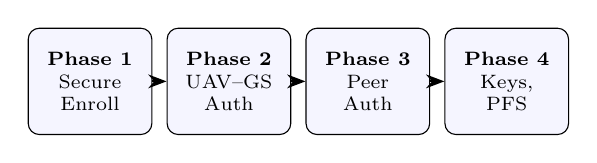
\begin{tikzpicture}[
  box/.style={draw,rounded corners,align=center,minimum height=1.35cm,
              minimum width=1.57cm,font=\scriptsize,fill=blue!4},
  >=Stealth,node distance=0.18cm]
\node[box] (p1) {\textbf{Phase 1}\\Secure\\Enroll};
\node[box,right=of p1] (p2) {\textbf{Phase 2}\\UAV--GS\\Auth};
\node[box,right=of p2] (p3) {\textbf{Phase 3}\\Peer\\Auth};
\node[box,right=of p3] (p4) {\textbf{Phase 4}\\Keys,\\PFS};
\draw[->,thick] (p1)--(p2); \draw[->,thick] (p2)--(p3); \draw[->,thick] (p3)--(p4);
\end{tikzpicture}
\caption{The four phases and what each produces. Enrollment is performed once,
in a secure facility; Phases 2 to 4 run in the field.}
\label{fig:overview}
\end{figure}

\subsection{Phase 1: secure enrollment and registration}
\label{sec:p1}

Enrollment runs once per drone, in a physically secure facility over a trusted
channel, before deployment. Its purpose is to establish the stable master key
$\text{mk}_i$ and the public helper data $P_i$, so that in the field the drone
can regenerate $\text{mk}_i$ from its own PUF without ever storing a secret.

\textbf{Step 1.1, PUF interrogation.} The GS draws a block of $L$ random
128-bit challenges and collects the concatenated enrollment response
\begin{equation}
R = \big(\mathrm{PUF}_i(C_i^{(1)}), \dots, \mathrm{PUF}_i(C_i^{(L)})\big).
\end{equation}
Concatenating $L$ blocks aggregates enough physical entropy to survive the
helper-data loss quantified in Lemma~\ref{lem:helper}.

\textbf{Step 1.2, key and helper-data generation.} The GS runs the
fuzzy-extractor generator $\mathsf{Gen}$ on $R$:
\begin{align}
c &= \mathsf{C}.\mathsf{Encode}(r), \quad r \xleftarrow{\$} \{0,1\}^{k}, &
s &= R \oplus c, \label{eq:gen}\\
\text{mk}_i &= \mathsf{KDF}(\mathsf{Ext}_{\text{seed}}(R); \texttt{root}), &
P_i &= (s, \text{seed}),
\end{align}
where $s$ is the public sketch that later lets a noisy response be decoded back
to $R$, and $\mathsf{Ext}$ is a strong extractor realised by the KDF.

\textbf{Step 1.3, sizing.} Because the sketch leaks at most $n-k = 124$ bits
per block, the block count $L$ must satisfy the entropy budget
\begin{equation}
\textstyle\sum_{b=1}^{L}\big(m_b - (n-k)\big) \;\ge\; \ell + 2\log_2(1/\varepsilon),
\label{eq:budget}
\end{equation}
where $m_b$ is the measured per-block min-entropy and $\varepsilon$ a negligible
statistical-distance target. This inequality is what makes $\text{mk}_i$ a
strong key rather than a slightly random one. A consequence worth stating
explicitly: because blocks must exceed the leak to contribute anything, blocks
are 255 bits, not the 128 bits of a native challenge--response pair. A 128-bit
block against a 124-bit leak contributes almost nothing at any block count.

\textbf{Step 1.4, identities and pair credentials.} The GS assigns a permanent
identity and an initial rotating temporary identity,
$\text{TID}_i = h(\text{ID}_i \|\text{seed}_i')$, and fixes a GS-only master key
from which all per-pair credentials are derived:
\begin{equation}
\text{Cred}_{ij} = \mathsf{KDF}\big(\text{mk}_{\text{GS}};\
\texttt{pair-cred} \| \min(i,j) \| \max(i,j)\big).
\end{equation}
The temporary identity hides the permanent one from eavesdroppers; each
$\text{Cred}_{ij}$ is a distinct secret for exactly one pair.

\textbf{Step 1.5, storage.} The GS stores
$\{\text{ID}_i, \text{TID}_i, \bm{C}_i, P_i, \text{mk}_i\}$ per drone plus
$\text{mk}_{\text{GS}}$, all in tamper-resistant memory. The drone stores
$\{\text{TID}_i, \bm{C}_i, P_i\}$ only, every one of which is public.
\emph{No secret is stored on the drone.} Capturing it yields no key material,
because $\text{mk}_i$ exists only transiently, regenerated from the PUF
whenever it is needed.

\subsection{Phase 2: UAV to Ground Station mutual authentication}
\label{sec:p2}

Phase~2 (Fig.~\ref{fig:phase2}) runs when a drone powers up in the field. It is
a four-message exchange that mutually authenticates the drone and the GS,
establishes a forward-secret session key, and delivers the drone's per-pair
credentials for Phase~3. Both sides key their MACs with
$K^{i}_{\text{auth}} = \mathsf{KDF}(\text{mk}_i;\texttt{p2-auth})$: the GS from
its stored record, the drone from its PUF.

\begin{figure}[H]
\centering
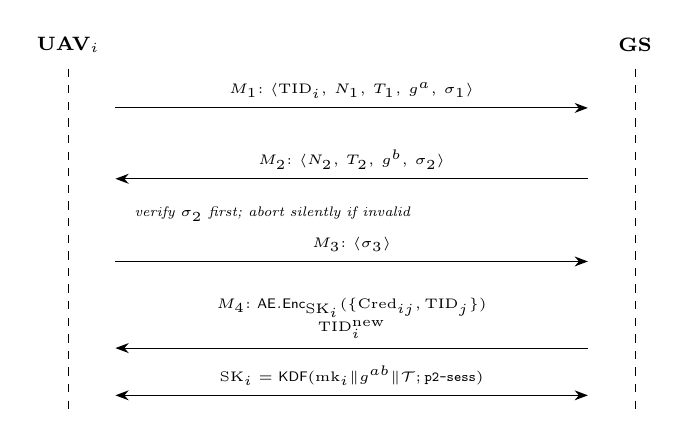
\begin{tikzpicture}[>=Stealth,font=\scriptsize]
  \node at (0,0) {\textbf{UAV$_i$}};
  \node at (7.2,0) {\textbf{GS}};
  \draw[dashed] (0,-0.3)--(0,-4.7);
  \draw[dashed] (7.2,-0.3)--(7.2,-4.7);
  \draw[->] (0.6,-0.8)--node[above,font=\tiny]{$M_1{:}\ \langle \text{TID}_i,\,N_1,\,T_1,\,g^{a},\,\sigma_1\rangle$}(6.6,-0.8);
  \draw[->] (6.6,-1.7)--node[above,font=\tiny]{$M_2{:}\ \langle N_2,\,T_2,\,g^{b},\,\sigma_2\rangle$}(0.6,-1.7);
  \node[font=\tiny,anchor=west] at (0.72,-2.15) {\emph{verify $\sigma_2$ first; abort silently if invalid}};
  \draw[->] (0.6,-2.75)--node[above,font=\tiny]{$M_3{:}\ \langle \sigma_3\rangle$}(6.6,-2.75);
  \draw[->] (6.6,-3.85)--node[above,font=\tiny,align=center]{$M_4{:}\ \mathsf{AE}.\mathsf{Enc}_{\text{SK}_i}(\{\text{Cred}_{ij},\text{TID}_j\})$\\$\text{TID}_i^{\text{new}}$}(0.6,-3.85);
  \draw[<->] (0.6,-4.45)--node[above,font=\tiny]{$\text{SK}_i=\mathsf{KDF}(\text{mk}_i\|g^{ab}\|\mathcal{T};\texttt{p2-sess})$}(6.6,-4.45);
\end{tikzpicture}
\caption{Phase-2 message sequence. The drone validates the GS authenticator
before it replies, so a fraudulent challenger draws no response, and peer
credentials ship under authenticated encryption only after mutual
authentication succeeds.}
\label{fig:phase2}
\end{figure}

\textbf{Message $M_1$, authentication request.} The drone regenerates
$\text{mk}_i$ (PUF evaluation plus $\mathsf{Rep}$), picks a fresh nonce and an
ephemeral scalar, and authenticates the opening message:
\begin{align}
N_1 &\xleftarrow{\$} \{0,1\}^{128}, \qquad a \xleftarrow{\$} \text{scalar},\\
\sigma_1 &= \mathsf{MAC}_{K^{i}_{\text{auth}}}\big(\texttt{m1} \| \text{TID}_i \| N_1 \| T_1 \| g^{a}\big),\\
M_1 &= \langle \text{TID}_i, N_1, T_1, g^{a}, \sigma_1 \rangle.
\end{align}
Since $\sigma_1$ is keyed by $K^{i}_{\text{auth}}$, only a party holding
$\text{mk}_i$, the genuine drone through its PUF, or the GS through its
database, can produce it. The type tag $\texttt{m1}$ stops a token from one
step being replayed as another.

\textbf{Message $M_2$, GS response.} The GS checks the timestamp and nonce for
freshness, looks up $\text{mk}_i$, verifies $\sigma_1$, and answers with its own
nonce and ephemeral share:
\begin{align}
N_2 &\xleftarrow{\$} \{0,1\}^{128}, \qquad b \xleftarrow{\$} \text{scalar},\\
\sigma_2 &= \mathsf{MAC}_{K^{i}_{\text{auth}}}\big(\texttt{m2} \| \text{TID}_i \| N_1 \| N_2 \| T_2 \| g^{a} \| g^{b}\big),\\
M_2 &= \langle N_2, T_2, g^{b}, \sigma_2 \rangle.
\end{align}
$\sigma_2$ authenticates the GS to the drone: it binds both nonces and both
ephemeral shares under the shared key, so no network adversary can forge or
alter it.

\textbf{Message $M_3$, drone confirmation.} The drone verifies $\sigma_2$
\emph{before it does anything else} and aborts silently if the check fails.
This verify-before-respond rule is what prevents a fraudulent GS from using the
drone as an oracle: an attacker who cannot forge $\sigma_2$ elicits no reply at
all. If the check passes, the drone confirms the transcript:
\begin{equation}
\sigma_3 = \mathsf{MAC}_{K^{i}_{\text{auth}}}\big(\texttt{m3} \| \mathcal{T}\big), \qquad
M_3 = \langle \sigma_3 \rangle,
\end{equation}
where $\mathcal{T}$ is the concatenation of all fields of $M_1$ and $M_2$. The
raw PUF response is consumed inside $\mathsf{Rep}$ and never appears on the
wire; only a MAC over public values is sent.

\textbf{Message $M_4$, credential delivery.} After verifying $\sigma_3$, both
parties hold the same ingredients and derive the forward-secret session key
\begin{equation}
\text{SK}_i = \mathsf{KDF}\big(\text{mk}_i \| g^{ab} \| \mathcal{T};\ \texttt{p2-sess}\big),
\label{eq:sk2}
\end{equation}
after which the GS delivers the drone's per-pair credentials and a fresh
identity under authenticated encryption:
\begin{align}
\text{CredPkg} &= \mathsf{AE}.\mathsf{Enc}_{\text{SK}_i}\big(\{(\text{Cred}_{ij}, \text{TID}_j)\}_{j \ne i}\big),\\
\text{TID}_i^{\text{new}} &= h(\text{TID}_i \| \text{mk}_i \| N_1 \| N_2),\\
M_4 &= \langle \text{CredPkg}, \text{TID}_i^{\text{new}} \rangle.
\end{align}
Authenticated encryption gives the credentials both confidentiality and
integrity. The session key mixes in $g^{ab}$, which is what makes it
forward-secret (Section~\ref{sec:p4}).

\subsection{Phase 3: UAV-to-UAV peer authentication}
\label{sec:p3}

Phase~3 lets any two drones that both completed Phase~2 authenticate each other
directly (Fig.~\ref{fig:phase3}) on the per-pair credential each received
encrypted. No GS involvement is needed, so peer authentication keeps working
when the command link is down. Both sides key their MACs with
$K^{ij}_{\text{auth}} = \mathsf{KDF}(\text{Cred}_{ij}; \texttt{peer-auth})$.

\begin{figure}[H]
\centering
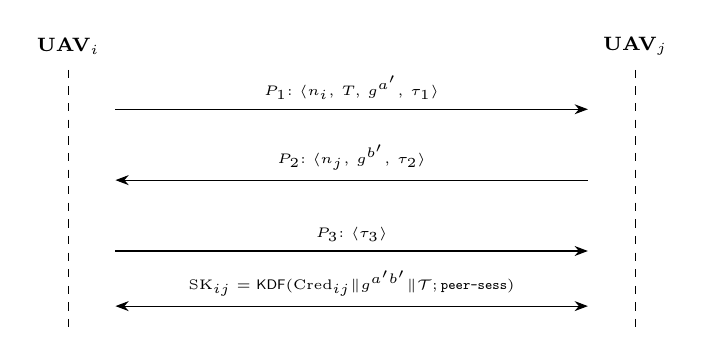
\begin{tikzpicture}[>=Stealth,font=\scriptsize]
  \node at (0,0) {\textbf{UAV$_i$}};
  \node at (7.2,0) {\textbf{UAV$_j$}};
  \draw[dashed] (0,-0.3)--(0,-3.6);
  \draw[dashed] (7.2,-0.3)--(7.2,-3.6);
  \draw[->] (0.6,-0.8)--node[above,font=\tiny]{$P_1{:}\ \langle n_i,\,T,\,g^{a'},\,\tau_1\rangle$}(6.6,-0.8);
  \draw[->] (6.6,-1.7)--node[above,font=\tiny]{$P_2{:}\ \langle n_j,\,g^{b'},\,\tau_2\rangle$}(0.6,-1.7);
  \draw[->] (0.6,-2.6)--node[above,font=\tiny]{$P_3{:}\ \langle \tau_3\rangle$}(6.6,-2.6);
  \draw[<->] (0.6,-3.3)--node[above,font=\tiny]{$\text{SK}_{ij}=\mathsf{KDF}(\text{Cred}_{ij}\|g^{a'b'}\|\mathcal{T};\texttt{peer-sess})$}(6.6,-3.3);
\end{tikzpicture}
\caption{Phase-3 message sequence. Every token is a MAC keyed by the per-pair
credential $\text{Cred}_{ij}$ and tagged with its message type, so tokens
cannot be reflected or reused across steps.}
\label{fig:phase3}
\end{figure}

\textbf{Message $P_1$, peer request.} The initiator picks a fresh nonce and
ephemeral share:
\begin{align}
\tau_1 &= \mathsf{MAC}_{K^{ij}_{\text{auth}}}\big(\texttt{p1} \| i \| j \| n_i \| T \| g^{a'}\big),\\
P_1 &= \langle n_i, T, g^{a'}, \tau_1 \rangle.
\end{align}
Because $\tau_1$ is keyed by $\text{Cred}_{ij}$, which only $\text{UAV}_i$ and
$\text{UAV}_j$ possess, a third party, even one holding some other pair's
credential, cannot produce it.

\textbf{Message $P_2$, peer response.} The responder verifies $\tau_1$, then
answers:
\begin{equation}
\tau_2 = \mathsf{MAC}_{K^{ij}_{\text{auth}}}\big(\texttt{p2} \| i \| j \| n_i \| n_j \| g^{a'} \| g^{b'}\big), \quad
P_2 = \langle n_j, g^{b'}, \tau_2 \rangle.
\end{equation}
$\tau_2$ binds both identities and both nonces, so it authenticates
$\text{UAV}_j$ to $\text{UAV}_i$ and confirms both are in the same fresh
session.

\textbf{Message $P_3$, completion.} The initiator verifies $\tau_2$ and closes
the handshake:
\begin{equation}
\tau_3 = \mathsf{MAC}_{K^{ij}_{\text{auth}}}\big(\texttt{p3} \| \mathcal{T}\big), \qquad
P_3 = \langle \tau_3 \rangle.
\end{equation}
The three distinct type tags rule out reflection. A full mesh over $N$ drones
runs $N(N-1)/2$ independent Phase-3 exchanges, 45 at $N=10$ and 190 at $N=20$,
all of which may proceed in parallel.

\subsection{Phase 4: session-key establishment and forward secrecy}
\label{sec:p4}

Phase~4 is the keying both interactive phases finish with. In Phase~2 the
UAV--GS key is $\text{SK}_i$ of Eq.~\eqref{eq:sk2}; in Phase~3 the peer key is
\begin{equation}
\text{SK}_{ij} = \mathsf{KDF}\big(\text{Cred}_{ij} \| g^{a'b'} \| \mathcal{T};\ \texttt{peer-sess}\big).
\label{eq:sk3}
\end{equation}
Both keys share one shape, written uniformly as
\begin{equation}
\text{SK} = \mathsf{KDF}\big(k_{\text{lt}} \| g^{xy} \| \mathcal{T};\ \ell\big),
\label{eq:sk}
\end{equation}
with $k_{\text{lt}} = \text{mk}_i$ or $\text{Cred}_{ij}$. Two independent
secrets go into every session key. The long-term one ties the session to the
PUF through $\text{mk}_i$ or to the pair through $\text{Cred}_{ij}$. The
ephemeral one, $g^{xy}$, whose public shares were authenticated inside the MAC
transcript of the handshake, is what provides perfect forward secrecy: once the
ephemeral scalars are erased, an adversary who later learns $k_{\text{lt}}$
still cannot reconstruct a past key, because doing so requires solving
Diffie--Hellman on the recorded shares. The exchange is mandatory, there is no
derivation path that omits $g^{xy}$, so a session either establishes a
forward-secret key or fails.

\subsection{Canonical message encoding}

One encoder produces the wire image, the input to the MAC, and the byte count
driving the link delay, so reported overhead cannot drift from what is actually
sent. Each field is a type tag, a two-byte length, and a value, under a header
carrying the protocol version, the suite identifier, and a per-message-type
tag:
\begin{align}
\mathsf{field}(t,v) &= \mathsf{u8}(t) \| \mathsf{u16}(|v|) \| v,\\
\mathsf{enc} &= \mathsf{u8}(\text{ver}) \| \mathsf{u8}(\text{suite}) \| \mathsf{u8}(\text{type}) \notag\\
&\qquad \| \mathsf{u16}(k) \| \mathsf{field}(t_1,v_1)\cdots
\end{align}
with tags emitted in strictly ascending order. The encoding is injective, no two
distinct field sets share a byte string, and canonical, each field set has
exactly one valid encoding, which is precisely the precondition the
unforgeability argument of Section~\ref{sec:security} requires of its MAC
inputs. Non-canonical input, duplicate or out-of-order tags, is rejected rather
than accepted.

%=============================================================================
\section{Security Analysis}
\label{sec:security}
%=============================================================================

The proofs rely on the following standard assumptions. (1) \textbf{Hash
security}: $h$ is pre-image, second-pre-image, and collision resistant, and is
modelled as a random oracle in the reductions. (2) \textbf{MAC
unforgeability}: $\mathsf{MAC}$ is existentially unforgeable under
chosen-message attack (EUF-CMA). (3) \textbf{AEAD security}: $\mathsf{AE}$
provides ciphertext indistinguishability (IND-CCA) and ciphertext integrity
(INT-CTXT). (4) \textbf{PUF unpredictability}: given polynomially many
challenge--response pairs, the response to a fresh challenge is computationally
indistinguishable from uniform to an adversary that does not possess the
device, and invasive probing destroys it. (5) \textbf{Diffie--Hellman}: the gap
computational Diffie--Hellman (gap-CDH) problem is hard in $\mathbb{G}$.

\subsection{Helper-data privacy}

\begin{lemma}[Helper-data privacy]
\label{lem:helper}
Let the enrollment response $R$ have conditional min-entropy
$\widetilde{H}_\infty(R) = m$. The code-offset sketch $s = R \oplus c$
discloses at most $n-k$ bits, so
\begin{equation}
\widetilde{H}_\infty(R \mid P) \;\ge\; m - (n-k).
\end{equation}
Consequently, if the extractor output length satisfies
$\ell \le m - (n-k) - 2\log_2(1/\varepsilon)$, then $\text{mk}$ is within
statistical distance $\varepsilon$ of uniform given the public helper data $P$.
\end{lemma}

\begin{IEEEproof}
Given the internal randomness $r$, the sketch pins $R$ to a coset of the
$[n,k]$ code $\mathsf{C}$, which fixes at most $n-k$ syndrome bits. The chain
rule for average min-entropy gives
$\widetilde{H}_\infty(R \mid s) \ge \widetilde{H}_\infty(R) - (n-k)$, and the
seed is independent of $R$. Applying the strong-extractor property to the
residual source yields a key within distance $\varepsilon$ of uniform.
\end{IEEEproof}

\subsection{Phase 2: mutual authentication}

\begin{theorem}[Phase-2 mutual authentication]
\label{thm:mutual}
After a successful Phase-2 exchange, $\text{UAV}_i$ and the GS have mutually
authenticated one another, and both agree on the transcript $\mathcal{T}$,
except with negligible probability.
\end{theorem}

\begin{IEEEproof}
Both directions rest on $K^{i}_{\text{auth}}$, which by Lemma~\ref{lem:helper}
and PUF unpredictability is unknown to any adversary lacking either the PUF or
the GS database, in the sense of the Bellare--Rogaway entity-authentication
framework~\cite{bellare_rogaway}. \emph{GS authenticates the drone:} the GS
accepts only if $\sigma_1$ and later $\sigma_3$ verify under $K^{i}_{\text{auth}}$;
producing a fresh valid tag without the key is exactly an EUF-CMA forgery.
\emph{Drone authenticates the GS:} symmetrically, the drone accepts only if
$\sigma_2$ verifies; although every field inside $\sigma_2$ is public, the
\emph{key} is secret, so a fresh valid $\sigma_2$ is again a forgery. A nonce
collision that could enable transcript reuse occurs with probability at most
$q^2/2^{128}$ for $q$ sessions. Absent forgery and collision, the two accepting
parties share identical fields in $M_1$ and $M_2$, hence agree on
$\mathcal{T}$.
\end{IEEEproof}

\begin{corollary}[No PUF read-out oracle]
\label{cor:oracle}
An adversary that impersonates the GS learns no PUF response, so it cannot
harvest challenge--response pairs to model the PUF.
\end{corollary}

\begin{IEEEproof}
By the verify-before-respond rule, the drone emits $M_3$ only after $\sigma_2$
verifies, which by Theorem~\ref{thm:mutual} an adversary can force only by
forging a MAC. On failure the drone sends nothing; on success the only value on
the wire is $\sigma_3$, a MAC over public transcript fields. The response is
consumed inside $\mathsf{Rep}$ and never transmitted, so no challenge--response
pair is exposed.
\end{IEEEproof}

\subsection{Replay and man-in-the-middle resistance}

\begin{theorem}[Replay resistance]
\label{thm:replay}
Phases 2 and 3 resist replay attacks.
\end{theorem}

\begin{IEEEproof}
Three mechanisms combine. Every message carries a fresh 128-bit nonce and a
timestamp verified within a window $\Delta T$, so a verbatim replay reuses a
stale nonce or timestamp and is rejected. Each MAC binds a per-message type
tag, $\texttt{m1}$ through $\texttt{p3}$, so a token cannot be accepted at
another step. From the second message onward each MAC binds the partner's
nonce, so a token from one session cannot be reused in another without producing
a mismatch, which by Theorems~\ref{thm:mutual} and \ref{thm:peer} would require
a forgery.
\end{IEEEproof}

\begin{theorem}[MITM resistance]
\label{thm:mitm}
The protocol resists active man-in-the-middle attacks in both Phase 2 and
Phase 3.
\end{theorem}

\begin{IEEEproof}
Every accepted message is a MAC or an authenticated ciphertext over a transcript
that includes fresh nonces, a timestamp, a type tag, and, from the second
message onward, the partner's nonce and ephemeral share. Altering any
covered field invalidates its tag, and forging a new tag requires the secret
key, EUF-CMA or INT-CTXT. By the agreement guarantees of
Theorems~\ref{thm:mutual} and \ref{thm:peer}, both endpoints therefore hold the
identical transcript, so an interposed adversary cannot sit undetected between
them.
\end{IEEEproof}

\subsection{Phase 3: peer mutual authentication}

\begin{theorem}[Peer mutual authentication]
\label{thm:peer}
After a successful Phase-3 exchange, $\text{UAV}_i$ and $\text{UAV}_j$ have
mutually authenticated one another, without GS involvement, and no per-pair
secret is exposed in transit.
\end{theorem}

\begin{IEEEproof}
$\text{Cred}_{ij}$ reaches each endpoint only inside the Phase-2 package
$\mathsf{AE}.\mathsf{Enc}_{\text{SK}_i}(\cdots)$; by INT-CTXT the adversary
cannot make a drone accept a substituted credential, and by IND-CCA it learns
nothing about $\text{Cred}_{ij}$. Given a secret $\text{Cred}_{ij}$, the tokens
$\tau_1,\tau_2,\tau_3$ are MACs under $K^{ij}_{\text{auth}}$; each binds both
identities and both nonces, so a fresh acceptance forces a matching computation
by the partner, otherwise an EUF-CMA forgery. Because credentials are
pair-specific, a third party holding some other $\text{Cred}_{k\ell}$ has no
information about $\text{Cred}_{ij}$ and cannot assert identity $i$ to $j$.
\end{IEEEproof}

\subsection{Session-key secrecy and forward secrecy}

\begin{theorem}[Session-key secrecy]
\label{thm:key}
For an adversary that corrupts neither endpoint of the target session, the
session key of Eq.~\eqref{eq:sk} is indistinguishable from uniform.
\end{theorem}

\begin{IEEEproof}
The key is $\mathsf{KDF}(k_{\text{lt}} \| g^{xy} \| \mathcal{T})$. Two
independent secrets protect it: the long-term key $k_{\text{lt}}$, that is,
$\text{mk}_i$ by Lemma~\ref{lem:helper} and PUF unpredictability, or
$\text{Cred}_{ij}$ by the IND-CCA delivery of Theorem~\ref{thm:peer}, and the
Diffie--Hellman secret $g^{xy}$. Modelling the KDF as a pseudorandom function,
replacing it by a random function is undetectable up to its PRF advantage; the
input $g^{xy}$ is unpredictable under gap-CDH given only the authenticated
shares $g^{x}, g^{y}$. Hence the output is uniform up to negligible terms.
\end{IEEEproof}

\begin{theorem}[Perfect forward secrecy]
\label{thm:pfs}
If the ephemeral scalars are erased after use, then revealing the long-term
secrets, $\text{mk}_i$, $\text{Cred}_{ij}$, or $\text{mk}_{\text{GS}}$,
\emph{after} a target session closes does not compromise that session's key.
\end{theorem}

\begin{IEEEproof}
A post-session reveal gives the adversary $k_{\text{lt}}$ but not the erased
scalars $x, y$. The key of Eq.~\eqref{eq:sk} still depends on $g^{xy}$, which
the adversary must now compute from the recorded, authenticated shares
$g^{x}, g^{y}$, a gap-CDH instance. Because the ephemeral exchange is
mandatory, there is no non-ephemeral key to fall back on. Hence past keys remain
indistinguishable from uniform.
\end{IEEEproof}

\subsection{Physical capture resistance}

\begin{theorem}[Physical capture resistance]
\label{thm:capture}
Capturing $\text{UAV}_k$ and reading its NVM does not let the adversary
impersonate any other UAV to the GS, nor impersonate any peer pair that does not
involve $k$. A captured node's peer exposure is limited to its own $N-1$ links.
\end{theorem}

\begin{IEEEproof}
The NVM of $\text{UAV}_k$ holds $\{\text{TID}_k, \bm{C}_k, P_k, \{\text{Cred}_{kj}\}_j\}$
plus any live session keys; all of $\text{TID}_k, \bm{C}_k, P_k$ are public.
Impersonating $\text{UAV}_m$, $m \ne k$, in a fresh Phase-2 needs
$K^{m}_{\text{auth}}$, hence $\text{mk}_m$, which is never stored, is not
recoverable from $k$'s silicon by tamper evidence, and is unpredictable by the
PUF assumption, so this reduces to a MAC forgery. Impersonating a pair
$(m,\ell)$ with $k \notin \{m,\ell\}$ needs
$\text{Cred}_{m\ell} = \mathsf{KDF}(\text{mk}_{\text{GS}}; \cdot)$, which is
independent of every captured $\text{Cred}_{kj}$ because the KDF inputs differ
and $\text{mk}_{\text{GS}}$ never leaves the GS. Only pairs that include $k$
share a captured credential, giving the stated $N-1$ exposure.
\end{IEEEproof}

\subsection{Symbolic verification}

The computational theorems are corroborated by a symbolic model in the Tamarin
prover~\cite{tamarin}, whose multiset-rewriting calculus expresses freshness,
stateful credential issuance, and device-compromise events natively. In the
model, $h$, $\mathsf{MAC}$, $\mathsf{AE}$, and $\mathsf{KDF}$ are function
symbols with the usual equational theory, each PUF is a private per-device
function, and helper data and all wire terms are public. The Dolev--Yao
adversary controls the network. Two extra rules model compromise: one reveals a
captured node's NVM, its identities, helper data, and per-pair credentials, but
neither its PUF nor its master key, and one reveals long-term secrets after a
session closes, for the forward-secrecy query. The prover discharges lemmas
that correspond one-to-one with the theorems above: injective agreement for
Phases 2 and 3, a no-replay lemma, a capture-isolation lemma, a
session-key-secrecy lemma, and a forward-secrecy lemma. The PUF's noise is
idealised as a noiseless private function, since error tolerance is the
computational correctness property of the fuzzy extractor, and confidential
delivery is abstracted by a symmetric encryption operator, leaving the
fine-grained secrecy argument to the computational analysis.

\subsection{Summary}

Table~\ref{tab:secsum} summarises the guarantees and the mechanism behind each.

\begin{table}[H]
\centering
\caption{Summary of security properties and the mechanism behind each}
\label{tab:secsum}
\scriptsize
\setlength{\tabcolsep}{2.6pt}
\begin{tabular}{@{}p{3.3cm}p{5.1cm}@{}}
\toprule
\textbf{Property} & \textbf{Result and mechanism} \\
\midrule
UAV--GS mutual auth. & Keyed MAC under PUF-derived $\text{mk}_i$ (Thm.~\ref{thm:mutual}) \\
No PUF read-out oracle & Verify-before-respond; response stays on-device (Cor.~\ref{cor:oracle}) \\
Replay resistance & Nonces $+$ timestamps $+$ type tags (Thm.~\ref{thm:replay}) \\
Peer mutual auth. & Per-pair credential $+$ keyed MAC (Thm.~\ref{thm:peer}) \\
MITM resistance & Transcript-binding MACs / AEAD (Thm.~\ref{thm:mitm}) \\
Session-key secrecy & KDF over long-term key and DH secret (Thm.~\ref{thm:key}) \\
Forward secrecy & Mandatory authenticated ephemeral DH (Thm.~\ref{thm:pfs}) \\
Capture resistance & No stored key; per-pair credentials (Thm.~\ref{thm:capture}) \\
Identity anonymity & Rotating temporary identities \\
\bottomrule
\end{tabular}
\end{table}

%=============================================================================
\section{Reference Implementation}
\label{sec:impl}
%=============================================================================

The framework is implemented in C++17 on OMNeT++~6.3: 8{,}585 lines in
\texttt{src/}, 656 lines in the INET track (\texttt{src\_inet/}), and 4{,}125
lines of tests. The code separates protocol logic from simulation machinery:
the classes implementing Phases 1 to 4 depend only on abstract crypto
interfaces and byte strings, with no reference to the simulation kernel, so the
entire four-phase exchange can be driven over an in-memory transport and
validated independently of the network model. A single transmission module owns
the link-delay model, so propagation, serialisation, processing delay, and
jitter are defined once; the same module provides the interception point the
adversary uses, and with no adversary present it forwards immediately, keeping
attack and baseline runs directly comparable.

\subsection{Cryptographic suites}

Two interoperable suites implement one abstract interface, selected by a single
parameter (Table~\ref{tab:suites}).

\begin{table}[H]
\centering
\caption{The two cryptographic profiles}
\label{tab:suites}
\scriptsize
\setlength{\tabcolsep}{2.2pt}
\begin{tabular}{@{}p{1.75cm}p{3.3cm}p{3.3cm}@{}}
\toprule
\textbf{Component} & \textbf{Profile \texttt{sha3}} & \textbf{Profile \texttt{spongent}} \\
\midrule
Hash $h(\cdot)$ & SHA3-256 truncated to 160 bits & SPONGENT-160/160/16 \\
MAC & HMAC-SHA3-256, 128-bit tag & keyed sponge, 128-bit tag \\
KDF & HKDF~\cite{hkdf}, extract-then-expand & one-pass sponge \\
AEAD & ChaCha20-Poly1305 & Ascon-128a v1.2~\cite{ascon} \\
Key exchange & X25519~\cite{curve25519} & X25519 \\
Hash/MAC level & 128-bit & 80-bit ($c=160$) \\
Provenance & OpenSSL 3.5 & vendored \\
\bottomrule
\end{tabular}
\end{table}

Three points require explicit statement. \emph{First}, HMAC is not applicable
to the sponge profile. HMAC is defined over a compression function of block
size $B$ and requires $|K| \le B$. For SPONGENT-160/160/16 the rate is 16 bits,
so the block is two bytes, smaller than any useful key, and hashing the key
first still exceeds it. The construction is undefined there, and any ad-hoc
substitution would carry no proof. The sponge profile therefore uses the
standard prefix keyed sponge underlying KMAC~\cite{sha3_standard}, which is
sound for a sponge and needs no nested structure: a sponge with non-zero
capacity is not length-extendable, so the nesting HMAC exists to prevent is
unnecessary. \emph{Second}, the sponge profile operates at the 80-bit level:
with capacity $c=160$ the keyed-sponge bound gives roughly $c/2 = 80$ bits,
matching the collision resistance of a 160-bit digest but deliberately
asymmetric with the 128-bit AEAD and key exchange. It is presented as a
constrained-hardware profile at that level, not as a 128-bit one. \emph{Third},
key derivation is domain-separated: distinct leading bytes separate hash, MAC,
and KDF modes even where they share a permutation, and every derived key
carries a unique label (\texttt{p2-auth}, \texttt{p2-sess},
\texttt{pair-cred}, \texttt{peer-auth}, \texttt{peer-sess},
\texttt{tid-rotate}), so a key minted for one purpose cannot be mistaken for
another.

All protocol randomness, nonces, ephemeral scalars, extractor seeds, enrollment
challenges, is drawn from a deterministic generator seeded from the simulator's
random-number stream. Ephemeral X25519 scalars are loaded from those bytes
rather than generated internally, so an entire run, including every ephemeral
key, is reproducible from its configured seed.

\subsection{BCH codec}
\label{sec:impl-bch}

The generator polynomial is formed as the product of the minimal polynomials of
$\alpha^1, \dots, \alpha^{2t}$ over the \emph{complete} conjugate closure of
each root. For $t=18$ over $\mathrm{GF}(2^8)$ the closure contains 124 roots,
giving $\deg g = 124$ with binary coefficients and therefore
\begin{equation}
\mathrm{BCH}(n{=}255,\ k{=}131,\ t{=}18), \qquad n-k = 124 \text{ parity bits}.
\end{equation}
Both properties are asserted at construction: a non-binary coefficient
indicates an incomplete closure, and the parity length is computed rather than
assumed. This matters because $k = 131 \ge 128$ is what allows a full response
block to be protected; taking the parity length as $mt = 144$ instead would give
$k = 111$ and silently leave the tail of every response uncovered. Decoding
proceeds by syndrome computation, Berlekamp--Massey, and a Chien search,
followed by a check that the corrected word has all-zero syndromes. Failure is
reported as failure: the decoder never returns the uncorrected input while
indicating success.

\subsection{Fuzzy-extractor parameterisation}

Enrollment applies $\mathsf{Gen}$ to $L$ blocks of $n=255$ bits; reproduction
applies $\mathsf{Rep}$ with the public helper data. The budget of
Eq.~\eqref{eq:budget} in the form
\begin{equation}
L\big(\rho n - (n-k)\big) \;\ge\; \ell + 2\log_2(1/\varepsilon)
\label{eq:budget2}
\end{equation}
is enforced at construction and raises an error when unmet, rather than being
documented and left to the caller. With $\rho = 0.95$, $\ell = 256$, and
$\varepsilon = 2^{-64}$, each block contributes $118.25$ bits and $L=4$ gives
$473 \ge 384$. Three profiles are provided (Table~\ref{tab:fe}). The default
uses the parameters of Section~\ref{sec:fe}; the third concatenates a
$[3,1,3]$ repetition inner code, which must operate on repeated measurements of
the same physical bit: enrollment fixes a reference and publishes each copy's
offset as additional helper data, and reproduction removes those offsets before
voting, reducing the per-bit error rate from $p$ to approximately $3p^2$. The
inner offsets are charged to the leak accounting at $(\mathrm{rep}-1)$ bits per
outer bit. Reproduction fails closed: if any block fails to decode, no key
material is returned.

\begin{table}[H]
\centering
\caption{Fuzzy-extractor profiles}
\label{tab:fe}
\scriptsize
\setlength{\tabcolsep}{2.2pt}
\begin{tabular}{@{}p{4.9cm}ccr@{}}
\toprule
\textbf{Profile (code)} & \textbf{$L$} & \textbf{PUF bits} & \textbf{Leak} \\
\midrule
\texttt{bch255-131-18}, default (BCH(255,131,18)) & 4 & 1020 & 496 \\
\texttt{bch255-91-25} (BCH(255,91,25)) & 5 & 1275 & 820 \\
\texttt{rep3-bch255-131-18}, $[3,1,3]{+}$BCH & 5 & 3825 & 3170 \\
\bottomrule
\end{tabular}
\end{table}

\subsection{PUF models}

Three models are provided and every result states which one it rests on. The
\emph{ideal} model realises the strong-PUF abstraction as a keyed pseudorandom
function and is used where near-uniform responses are the intended assumption.
The \emph{arbiter} model implements the additive-delay formulation over 128
stages with per-device Gaussian delay weights. The \emph{xor-arbiter} model
XORs $k$ arbiter chains.

Both models return a whole response from one keyed stream rather than one
evaluation per bit. The ideal model is the concatenation of successive 256-bit
blocks,
\begin{equation}
R = \mathsf{HMAC}_{\text{SHA3-256}}\big(k_{\text{dev}},\ \ell \,\|\, C \,\|\, n\big)_{n \ge 0}
    \ \big|_{\le b\ \text{bits}},
\end{equation}
truncated to the response length $b$, so four calls cover the 1020-bit response
the default profile requires; the arbiter model draws all of its per-bit
sub-challenges from one analogous $\mathsf{SHA3\text{-}256}$ stream. This is a
simulation-cost decision with no cryptographic consequence, the object remaining
the same keyed PRF per device with independent uniform output bits, but
evaluating each bit separately cost two hash calls per bit and made the
simulated PUF the slowest part of a protocol whose real device answers in
nanoseconds. Response noise is applied as a 16-bit threshold on two
pseudorandom bytes per bit, an exact Bernoulli($p$) channel to 16-bit precision,
with the same two bytes drawn whatever $p$ is, so a run stays reproducible when
that setting changes.

In the arbiter model, measurement noise is added to the
accumulated delay \emph{difference} rather than by flipping output bits:
\begin{equation}
\Delta' = \textstyle\sum_{i} w_i \phi_i + \mathcal{N}(0,\sigma), \qquad
r = \mathbb{1}[\Delta' > 0].
\end{equation}
Bits whose delay difference sits near zero therefore flip far more often than
the rest, reproducing the reliability profile of real silicon: the measured
variance of per-bit flip rates is approximately $98\times$ that of a uniform
bit-flip channel, a structural property a per-bit model cannot exhibit. A
calibration routine converts a target average bit-error rate into the matching
$\sigma$. Measured over 24 devices and 276 device pairs, inter-device Hamming
distance is $0.5019$ (arbiter) and $0.5026$ (ideal), consistent with the ideal
$0.5$, and calibrated bit-error rates track their targets within 0.2 percentage
points across 1\% to 10\%.

\subsection{Verification of primitives}

Each primitive is checked against published reference values where they exist,
and reports its verification status programmatically (Table~\ref{tab:kat}).

\begin{table}[H]
\centering
\caption{Verification evidence per primitive}
\label{tab:kat}
\scriptsize
\setlength{\tabcolsep}{2.2pt}
\begin{tabular}{@{}p{2.5cm}p{6.1cm}@{}}
\toprule
\textbf{Primitive} & \textbf{Evidence} \\
\midrule
SHA3-256 & FIPS 202 / CAVP short-message vectors \\
HMAC-SHA3-256 & NIST example values with intermediate results \\
HKDF & RFC 5869, Appendices A.1 to A.3 \\
ChaCha20-Poly1305 & RFC 8439, Section 2.8.2 \\
X25519 & RFC 7748, Section 6.1; low-order points rejected \\
Ascon-128a & all 1089 vectors of the official LWC known-answer-test file \\
SPONGENT-160 & byte-exact against the designers' reference implementation and the
published digest; no official KAT file exists, and none is claimed \\
BCH(255,131,18) & $\deg g = 124$; $g(x) \mid x^{255}+1$; exact recovery in all
18{,}000 trials across weights 1 to 18; failure correctly reported beyond the
radius in 3{,}000 trials \\
\bottomrule
\end{tabular}
\end{table}

Neither vendored primitive has undergone timing or side-channel analysis. Tag
comparisons use a constant-time routine and no branch depends on secret data,
but nothing stronger is claimed, and the verification-status strings say so; a
regression test fails if that qualification is removed. The unit suite
comprises twelve test programs with approximately $4.3\times10^{5}$ assertions,
covering the primitives above, the encoding, the fuzzy extractor, the PUF
models, both signature baselines, and the full four-phase exchange.

\subsection{Simulation model}
\label{sec:impl-sim}

The scenario places $N$ UAVs around a $500\times300$~m field with the GS at its
centre. Link delay is the sum of propagation from node coordinates,
serialisation at the configured bit rate of 6~Mbps, a fixed processing delay of
0.1~ms, and half-normal jitter with standard deviation 0.02~ms, each reported
separately per message. This primary model does not itself simulate MAC-layer
contention, so its network delay is a lower bound; Section~\ref{sec:inet}
reports a second, independent measurement of the same Phase-2 handshake over a
real IEEE~802.11 stack with genuine CSMA/CA contention, so the lower bound is
bracketed from above rather than left undisclosed. All node parameters are
declared with defaults and are overridable from the configuration file, and
statistics are declared so that scalar and vector outputs are recorded.

\subsection{Evaluation scenarios}

Every scenario in Section~\ref{sec:eval} changes exactly one variable relative
to the reference configuration \texttt{StadiumSHA3} and holds everything else
fixed, so a difference in outcome can be attributed to that one variable and not
to a confound. Table~\ref{tab:scenarios} lists all sixteen configurations,
the single variable each isolates, and where each result is reported.

\begin{table}[H]
\centering
\caption{Evaluation scenarios, the single variable each isolates, and where
its result is reported}
\label{tab:scenarios}
\scriptsize
\setlength{\tabcolsep}{1.2pt}
\begin{tabular}{@{}>{\ttfamily\tiny}p{2.5cm}p{3.9cm}p{2.2cm}@{}}
\toprule
\normalfont\textbf{Scenario} & \textbf{Variable isolated and effect measured} &
\textbf{Reported in} \\
\midrule
StadiumSHA3 & reference point, $N{=}10$, software suite & Tabs.\ \ref{tab:functional}--\ref{tab:inet} \\
StadiumSPONGENT & crypto suite swap & Tabs.\ \ref{tab:msg}--\ref{tab:latency} \\
Baseline5UAV & swarm size $N{=}5$, lower scaling end & Tab.\ \ref{tab:latency} \\
Swarm20 & $N{=}20$; per-pair cost stays flat & Tab.\ \ref{tab:latency} \\
ArbiterPuf & arbiter PUF model, 3\% BER & Tab.\ \ref{tab:functional} \\
HighNoise & BER forced to 5\%, reliability edge & Tab.\ \ref{tab:functional} \\
NoiseSweep & BER 1--10\%, three FE profiles & Tab.\ \ref{tab:noise} \\
Inet80211SHA3 & real 802.11 CSMA/CA contention, Phase 2 and Phase 3 & Tab.\ \ref{tab:inet} \\
InetMobilityLinearSHA3 & same, drones moving linearly & Tab.\ \ref{tab:inet} \\
InetMobilityRandomWalkSHA3 & same, random-waypoint motion & Tab.\ \ref{tab:inet} \\
BaselineRSA & RSA-2048 baseline comparison & Tab.\ \ref{tab:baseline} \\
BaselineECDSA & ECDSA-P256 baseline comparison & Tab.\ \ref{tab:baseline} \\
AtkGsImpersonate & forged GS challenge, oracle resistance & Tab.\ \ref{tab:attacks} \\
AtkLegacyGsImpersonate & same attacker, P3 removed & Tab.\ \ref{tab:attacks} \\
AtkReplayM1 & $M_1$ replay within the window & Tab.\ \ref{tab:attacks} \\
AtkCredentialSniff & passive read of $M_4$ & Tab.\ \ref{tab:attacks} \\
\bottomrule
\end{tabular}
\end{table}

%=============================================================================
\section{Performance Evaluation}
\label{sec:eval}
%=============================================================================

All runs execute on an AMD Ryzen 5 5625U with OpenSSL 3.5.5 and
OMNeT++~6.3 (git commit 0e415cb). Each configuration runs thirty independent
repetitions with distinct seed sets, five for the attack configurations,
individually justified in Section~\ref{sec:attacks}.

\subsection{Methodology}
\label{sec:method}

The unit of replication is the \emph{run}, not the individual record:
observations inside one run share a pseudorandom stream and a single scheduling
epoch, so they are correlated. Confidence intervals are therefore computed in
two stages, a per-run mean followed by a $t$-interval across run means with
$R-1$ degrees of freedom. Pooling all records instead would inflate the degrees
of freedom from $R-1$ to $NR-1$ and understate every interval by roughly
$\sqrt{N}$. Intervals are reported as mean $\pm$ half-width at 95\%, and the
analysis refuses to form an interval from fewer than three runs. Proportions
carry Wilson score intervals, which behave correctly near 0 and 1; where no
failure is observed, the rule-of-three upper bound applies, so 100 successes in
100 trials bounds the failure probability at about 3\% and is reported as such,
not as perfection.

Compute times are host wall-clock measurements; network delays are simulated.
These are distinct clocks and are reported separately, never summed without
qualification. Simulated elapsed time is a third quantity: the OMNeT++ clock's
own start-to-finish reading for the handshake, which does not advance while
host compute is being measured, so it is close to the network column and
systematically smaller than Compute $+$ Network. Where one realistic figure is
wanted, this paper uses Compute $+$ Network and says so. Per-primitive costs
are measured over batches of at least $10^3$ iterations and reported as
medians, since a single clock read of tens of nanoseconds is not negligible
against a microsecond-scale operation.

\subsection{Functional correctness}
\label{sec:eval-fun}

Table~\ref{tab:functional} reports authentication outcomes. Two success rates
are distinguished because they answer different questions: one counts drones
that transmitted a first message, the other counts all enrolled devices. They
diverge when a drone cannot reproduce its master key, in which case it never
initiates at all, and reporting only the first would conceal that failure mode
entirely.

\begin{table}[H]
\centering
\caption{Authentication outcomes, thirty repetitions per configuration}
\label{tab:functional}
\scriptsize
\setlength{\tabcolsep}{2.6pt}
\begin{tabular}{@{}lccccc@{}}
\toprule
\textbf{Configuration} & \textbf{Dev.} & \textbf{Auth.} & \textbf{Rate} &
\textbf{Wilson 95\%} & \textbf{Pairs} \\
\midrule
StadiumSHA3 ($N{=}10$)      & 300 & 300 & 1.000 & [0.987, 1.000] & 2700/2700 \\
StadiumSPONGENT ($N{=}10$)  & 300 & 300 & 1.000 & [0.987, 1.000] & 2700/2700 \\
Baseline5UAV ($N{=}5$)      & 150 & 150 & 1.000 & [0.975, 1.000] & 600/600 \\
Swarm20 ($N{=}20$)          & 600 & 600 & 1.000 & [0.994, 1.000] & 11400/11400 \\
ArbiterPuf (3\% BER)        & 300 & 298 & 0.993 & [0.976, 0.998] & 2664/2690 \\
HighNoise (5\% BER)         & 300 & 247 & 0.823 & [0.776, 0.862] & 1830/2214 \\
\bottomrule
\end{tabular}
\end{table}

With the ideal PUF model, every device authenticates in every configuration,
including the twenty-drone swarm where all 11{,}400 peer-pair views complete.
Under the arbiter model at 3\% bit-error rate, two devices in three hundred
fail to regenerate their key; at 5\%, fifty-three do. Those failures are
reliability limits of the fuzzy extractor, not authentication failures, and are
analysed in Section~\ref{sec:reliability}.

\subsection{Latency and communication cost}

\begin{table}[H]
\centering
\caption{Phase-2 latency and overhead (mean $\pm$ 95\% CI, thirty runs).
Compute and Network are independent measurements on two clocks, never silently
summed; their sum is the realistic total. The PUF-noise configurations are
reported in Table~\ref{tab:noise} instead}
\label{tab:latency}
\scriptsize
\setlength{\tabcolsep}{2.4pt}
\begin{tabular}{@{}lccc@{}}
\toprule
\textbf{Configuration} & \textbf{Compute} &
\textbf{Network} & \textbf{Bytes} \\
 & \textbf{(ms)} & \textbf{(ms)} & \\
\midrule
StadiumSHA3     & $0.569{\pm}0.036$ & $1.074{\pm}0.002$ & 777 \\
StadiumSPONGENT & $3.456{\pm}0.102$ & $1.079{\pm}0.002$ & 781 \\
Baseline5UAV    & $0.458{\pm}0.003$ & $0.714{\pm}0.003$ & 507 \\
Swarm20         & $0.487{\pm}0.023$ & $1.790{\pm}0.006$ & 1315 \\
\bottomrule
\end{tabular}
\end{table}

Compute varies by nearly $6\times$ across the two suites while network delay is
identical to four significant figures, because the link model depends only on
message size and position, neither of which the suite changes.

Phase-3 peer authentication costs $0.4166 \pm 0.0006$~ms per pair with 197~bytes
of traffic, pooled across the four configurations that vary swarm size
(StadiumSHA3, StadiumSPONGENT, Baseline5UAV, Swarm20; the PUF-noise
configurations are excluded from this particular figure since they hold $N$
fixed and vary bit-error rate instead). The per-configuration means, $0.4171$,
$0.4171$, $0.4163$, and $0.4159$~ms respectively, agree to within their own
confidence intervals, so the pooled figure is independent of swarm size: the
$O(N^2)$ growth in total cost comes entirely from the pair count, not from a
per-pair cost that grows with $N$.

Phase-2 overhead grows with $N$ because the credential package in $M_4$ carries
one per-pair credential per peer: 275~B at $N=5$, 545~B at $N=10$, and
1{,}085~B at $N=20$, against a fixed 232~B for $M_1$ to $M_3$. An on-demand
variant issuing credentials per request is a straightforward extension where
this matters.

\subsection{Message-by-message breakdown}

Table~\ref{tab:msg} splits the handshake into its four messages under both
suites, reporting compute on each side, network delay, and wire size, averaged
over the full thirty-run, three-hundred-drone sample per suite.

\begin{table}[H]
\centering
\caption{Phase-2 message-by-message breakdown, \texttt{StadiumSHA3} versus
\texttt{StadiumSPONGENT}, mean over 300 handshakes per suite}
\label{tab:msg}
\tiny
\setlength{\tabcolsep}{2pt}
\begin{tabular}{@{}p{0.8cm}p{4.3cm}rrrr@{}}
\toprule
\textbf{Msg.} & \textbf{What it does} & \textbf{\texttt{sha3} (ms)} &
\textbf{\texttt{spg} (ms)} & \textbf{Net (ms)} & \textbf{B} \\
\midrule
$M_1$ & UAV: PUF eval.\ $+$ \texttt{Rep} $+$ MAC $\sigma_1$ & 0.3703 & 0.9323 & 0.2554 & 104 \\
      & \quad of which PUF evaluation & 0.0421 & 0.0405 & --- & --- \\
      & \quad of which BCH decode & 0.2452 & 0.5123 & --- & --- \\
      & GS: MAC $\sigma_1$ verify & 0.0595 & 0.6113 & --- & --- \\
$M_2$ & UAV: MAC $\sigma_2$ verify (the gate) & 0.0934 & 1.1953 & 0.2303 & 85 \\
$M_3$ & UAV: MAC $\sigma_3$ compute & 0.0934 & 1.1953 & 0.1737 & 43 \\
      & GS: MAC $\sigma_3$ verify $+$ sess.\ KDF & 0.1576 & 2.4677 & --- & --- \\
$M_4$ & GS: AEAD-seal credentials & 0.0122 & 0.1335 & 0.843/0.849 & 545/549 \\
\midrule
\textbf{Total} & & \textbf{0.569} & \textbf{3.456} & \textbf{1.074/1.079} & \textbf{777/781} \\
\bottomrule
\end{tabular}
\end{table}

Three things stand out that the summary figures do not show on their own.
\emph{First}, $M_1$ carries the largest single cost, and it is not the PUF:
under \texttt{sha3} BCH reproduction alone is $0.245$~ms, which is 66\% of
$M_1$'s own compute
and 43\% of the entire handshake, while the PUF evaluation is $0.042$~ms. The
drone needs $\text{mk}_i$ to
authenticate $M_1$ itself, so \texttt{Rep} necessarily runs before $M_1$ is
sent, and $M_1$, not $M_3$, carries the PUF cost in the measured breakdown.
\emph{Second}, network delay is identical across suites to four significant
figures, because the link-delay model depends only on message size and node
position, neither of which the suite changes materially, so the entire
$1.60$~ms against $4.45$~ms compute gap, a factor of $2.78$, is attributable to
the crypto suite alone. \emph{Third}, the suite gap concentrates in $M_2$ and
$M_3$: each performs one MAC with no PUF or AEAD work beside it, so the
\texttt{spongent} keyed sponge costs roughly $14.6\times$ \texttt{sha3}'s HMAC
there, consistent with the per-call figures of Table~\ref{tab:prim}, while
$M_4$'s AEAD-only cost barely differs, Ascon-128a not being slower than
ChaCha20-Poly1305 in this implementation.

Table~\ref{tab:p3msg} performs the same decomposition for the three-message
peer handshake, pooled over 2{,}700 pair-views per suite.

\begin{table}[H]
\centering
\caption{Phase-3 message-by-message breakdown, mean over 2{,}700 pair-views per
suite}
\label{tab:p3msg}
\tiny
\setlength{\tabcolsep}{2.2pt}
\begin{tabular}{@{}p{0.8cm}p{4.85cm}rrr@{}}
\toprule
\textbf{Msg.} & \textbf{What it does} & \textbf{\texttt{sha3} (ms)} &
\textbf{\texttt{spg} (ms)} & \textbf{Net (ms)} \\
\midrule
$P_1$ & UAV$_i$: MAC $\tau_1$ compute (initiator) & 0.0223 & 0.1645 & 0.1214 \\
$P_2$ & UAV$_j$: verify $\tau_1$ $+$ MAC $\tau_2$ & 0.0239 & 0.2791 & 0.1107 \\
$P_3$ & UAV$_i$: verify $\tau_2$ $+$ MAC $\tau_3$ $+$ sess.\ KDF & 0.0402 & 0.5241 & 0.0743 \\
\midrule
\textbf{Total} (compute $+$ net) & & \textbf{0.393} & \textbf{1.274} & \\
\bottomrule
\end{tabular}
\end{table}

No Phase-3 message touches the PUF or the fuzzy extractor at all: every
microsecond in Table~\ref{tab:p3msg} is a MAC, a KDF, or an ephemeral
Diffie--Hellman operation on the already-delivered credential $\text{Cred}_{ij}$.
That is why Phase-3 compute, $0.104$~ms under \texttt{sha3}, is roughly a
fifth of Phase-2's $0.569$~ms: Phase 3 never re-pays the PUF or the
error-correction cost that dominates $M_1$. The \texttt{spongent} Phase-3
compute of $1.013$~ms is $9.7\times$ \texttt{sha3}'s, a wider relative gap than
Phase-2's $6.1\times$, because Phase 3 has no PUF or AEAD cost to dilute the
three consecutive MAC calls that dominate it.

\subsection{Primitive costs against public-key baselines}

Table~\ref{tab:prim} places two measurements side by side, both taken on the
same host, the same OpenSSL 3.5 build, and the same clock: the median per-call
cost of every primitive in this work's own two suites, measured in-protocol
inside the running simulation, and the median cost of RSA-2048, ECDSA P-256,
ECDH P-256, and X25519, measured under a dedicated tight-loop benchmark against
the same library.

\begin{table}[H]
\centering
\caption{Primitive-level cost: this work in-protocol and public-key baselines
in a dedicated benchmark, same host and library throughout}
\label{tab:prim}
\footnotesize
\setlength{\tabcolsep}{4.2pt}
\begin{tabular}{@{}llcc@{}}
\toprule
\multicolumn{4}{@{}l}{\textit{This work, measured in-protocol (median $\mu$s per call)}} \\
\textbf{Operation} & & \textbf{\texttt{sha3}} & \textbf{\texttt{spongent}} \\
\midrule
Hash$^{\ddagger}$ & & 1.00 & --- \\
MAC & & 2.41 & 224.82 \\
MAC verify & & 2.20 & 231.02 \\
KDF & & 5.51 & 132.71 \\
Extract & & 3.42 & 291.20 \\
AEAD seal & & 2.66 & 1.64 \\
AEAD open & & 1.58 & 1.47 \\
X25519 keygen$^{\dagger}$ & & 36.85 & 33.87 \\
X25519 derive$^{\dagger}$ & & 71.63 & 65.05 \\
\midrule
\multicolumn{4}{@{}l}{\textit{Public-key baselines, dedicated tight-loop benchmark}} \\
\textbf{Scheme} & \textbf{Operation} & \textbf{Median ($\mu$s)} & \textbf{Mean ($\mu$s)} \\
\midrule
RSA-2048 & sign & 530.3 & 541.7 \\
RSA-2048 & verify & 16.9 & 17.3 \\
ECDSA P-256 & sign & 20.4 & 21.3 \\
ECDSA P-256 & verify & 57.2 & 57.8 \\
ECDH P-256 & derive & 51.7 & 55.5 \\
X25519 & keygen$^{\dagger}$ & 36.1 & 42.9 \\
X25519 & derive$^{\dagger}$ & 64.1 & 64.8 \\
\bottomrule
\end{tabular}

\vspace{2pt}
\raggedright\scriptsize
$^{\dagger}$X25519 is measured twice on purpose, since it is the one operation
both blocks share. Both measurements call the identical code; the roughly
twofold gap, 34 to 65~$\mu$s in-protocol against 66 to 126~$\mu$s benchmarked,
is a measurement-context effect, ten calls interleaved with a simulated
handshake versus a 2000-iteration tight loop, not two implementations. The
benchmarked figure is used wherever this work's X25519 cost is compared against
the ECDH and ECDSA rows, since only figures taken under identical tight-loop
conditions are directly comparable; the in-protocol figure is used when
accounting for the measured Compute column of Table~\ref{tab:latency}.
$^{\ddagger}$Hash is not measured in-protocol because the running protocol never
calls a standalone hash at top level, it is always invoked inside
\texttt{mac}, \texttt{kdf}, or \texttt{extract}, so no in-protocol call count
exists for it. The figure is the same dedicated-benchmark measurement as the
public-key rows, included for completeness.
\end{table}

\begin{figure}[H]
\centering
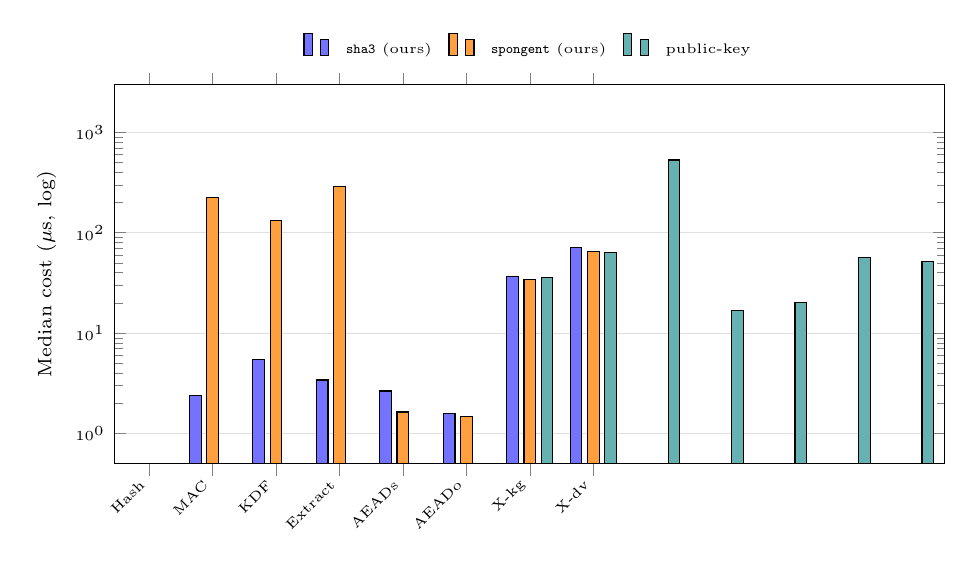
\begin{tikzpicture}
\begin{axis}[
  ybar, bar width=4.2pt, width=\linewidth, height=6.4cm,
  ymode=log, log origin=infty, ymin=0.5, ymax=3000,
  ylabel={Median cost ($\mu$s, log)}, ylabel style={font=\scriptsize},
  symbolic x coords={Hash,MAC,KDF,Extract,AEADs,AEADo,X-kg,X-dv,
    RSAs,RSAv,ECDSA-s,ECDSA-v,ECDHd},
  xtick=data, x tick label style={rotate=45,anchor=east,font=\tiny},
  ytick={1,10,100,1000}, yticklabel style={font=\tiny},
  enlarge x limits=0.045, ymajorgrids, grid style={gray!25},
  legend style={at={(0.5,1.04)},anchor=south,legend columns=3,font=\tiny,
                draw=none,column sep=4pt},
  ]
\addplot[fill=blue!55] coordinates
  {(Hash,0.49) (MAC,2.41) (KDF,5.51) (Extract,3.42) (AEADs,2.66) (AEADo,1.58)
   (X-kg,36.85) (X-dv,71.63)};
\addplot[fill=orange!75] coordinates
  {(MAC,224.82) (KDF,132.71) (Extract,291.20) (AEADs,1.64) (AEADo,1.47)
   (X-kg,33.97) (X-dv,64.56)};
\addplot[fill=teal!60] coordinates
  {(RSAs,530.3) (RSAv,16.9) (ECDSA-s,20.4) (ECDSA-v,57.2) (ECDHd,51.7)
   (X-kg,36.1) (X-dv,64.1)};
\legend{\texttt{sha3} (ours),\texttt{spongent} (ours),public-key}
\end{axis}
\end{tikzpicture}
\caption{Median per-call cost, this work's own primitives against public-key
baselines, one logarithmic axis (Table~\ref{tab:prim}). No bar is drawn for
\texttt{spongent} Hash, matching the dash in the table: HMAC's nested structure
is not defined over SPONGENT's two-byte rate, so the sponge profile
authenticates via a keyed sponge rather than a standalone hash call.}
\label{fig:prim}
\end{figure}

Three observations follow from Fig.~\ref{fig:prim}. \emph{First}, every
\texttt{sha3}-suite symmetric primitive is cheaper than every measured
asymmetric baseline: the most expensive, KDF at $5.5~\mu$s, is several times
below the cheapest baseline shown, RSA-2048 verify at $16.9~\mu$s. This
is a fair comparison because both sides are single, isolated primitive calls
measured the same way. \emph{Second}, the \texttt{spongent} suite does not
carry that advantage: its MAC, KDF, and Extract operations at $133$ to
$291~\mu$s land above the asymmetric baselines at $17$ to $64~\mu$s rather
than below them, the direct and disclosed cost of
a hardware-area-optimised permutation running in software, and a cost that does
not undercut the area argument that motivates the profile. Only the AEAD
operations stay cheap in both suites, $1.5$ to $1.6~\mu$s via Ascon.
\emph{Third}, neither of the previous readings is a claim about the full
protocol; both are single-primitive comparisons, one MAC call against one
signature verification. Section~\ref{sec:baseline} reports the full-protocol
comparison. Two further facts deserve notice, since they correct figures
sometimes repeated in the literature: RSA-2048 verification costs approximately
$17~\mu$s on this host, so millisecond-scale figures for that operation, and
protocol-level speedup multipliers built on them, are off by two to three
orders of magnitude; and this work's own mandatory ephemeral exchange, X25519
keygen plus derive at roughly $100~\mu$s under the like-for-like figure, is
comparable to an ECDH or ECDSA exchange at $52$ to $78~\mu$s, not faster by an
order of magnitude, which is the direct cost of making the exchange mandatory.
A protocol without it would be cheaper and would not offer forward secrecy.

\subsection{Full-protocol comparison against RSA and ECDSA baselines}
\label{sec:baseline}

Two real baseline protocols were built and run through the same simulator,
host, OpenSSL build, and link-delay model as this work's own Phase 2: a
signature-authenticated ephemeral X25519 exchange, one using RSA-2048 and one
using ECDSA P-256 in place of the PUF-derived MAC that authenticates
$M_1$ to $M_4$. Each is a genuine four-message mutual handshake $B_1$ to $B_4$
mirroring $M_1$ to $M_4$'s shape: the initiator signs its nonce and ephemeral
share, the responder verifies that signature \emph{before} doing anything else,
the same verify-before-respond discipline Theorem~\ref{thm:mutual} relies on,
replies with its own signed nonce and share, and both sides derive a session
key from the completed exchange and confirm it with a symmetric MAC. That is
the division of labour TLS~1.3 uses, a signature authenticates the exchange and
a MAC-based Finished message confirms the derived key, so neither baseline is a
straw-man construction. Long-term keypairs are provisioned once, out of band,
exactly as this work's own PUF challenge and helper data are provisioned in
Phase 1.

\begin{table}[H]
\centering
\caption{Full-protocol latency and overhead, RSA and ECDSA baselines versus
this work (mean $\pm$ 95\% CI, thirty runs each)}
\label{tab:baseline}
\scriptsize
\setlength{\tabcolsep}{1.7pt}
\begin{tabular}{@{}p{2.45cm}cccc@{}}
\toprule
\textbf{Protocol} & \textbf{Compute} &
\textbf{Network} & \textbf{Bytes} \\
 & \textbf{(ms)} & \textbf{(ms)} & \\
\midrule
RSA-2048 signed eph.\ DH   & $1.069{\pm}0.005$ & $0.699{\pm}0.002$ & 703 \\
ECDSA-P256 signed eph.\ DH & $0.341{\pm}0.005$ & $0.452{\pm}0.002$ & 333 \\
\midrule
This work (\texttt{sha3})     & $0.569{\pm}0.036$ & $1.074{\pm}0.002$ & 777 \\
This work (\texttt{spongent}) & $3.456{\pm}0.102$ & $1.079{\pm}0.002$ & 781 \\
\bottomrule
\end{tabular}
\end{table}

\begin{figure}[H]
\centering
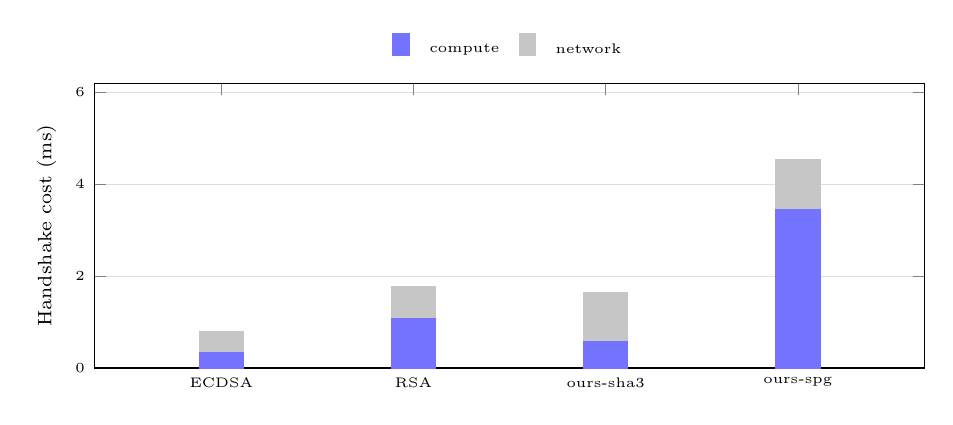
\begin{tikzpicture}
\begin{axis}[
  ybar stacked, bar width=16pt, width=\linewidth, height=5.2cm,
  ymin=0, ymax=6.2, ylabel={Handshake cost (ms)},
  ylabel style={font=\scriptsize}, yticklabel style={font=\tiny},
  symbolic x coords={ECDSA,RSA,{ours-sha3},{ours-spg}},
  xtick=data, x tick label style={font=\tiny},
  enlarge x limits=0.22, ymajorgrids, grid style={gray!25},
  legend style={at={(0.5,1.05)},anchor=south,legend columns=2,font=\tiny,
                draw=none,column sep=5pt},
  ]
\addplot[fill=blue!55,draw=blue!55] coordinates
  {(ECDSA,0.3410) (RSA,1.0685) ({ours-sha3},0.5693) ({ours-spg},3.4564)};
\addplot[fill=gray!45,draw=gray!45] coordinates
  {(ECDSA,0.4523) (RSA,0.6990) ({ours-sha3},1.0737) ({ours-spg},1.0790)};
\legend{compute,network}
\end{axis}
\end{tikzpicture}
\caption{Full-handshake Compute $+$ Network against real signature-authenticated
baselines (Table~\ref{tab:baseline}). Against ECDSA this work is genuinely
slower, $0.79$ against $1.64$~ms; against RSA it comes out marginally ahead,
$1.64$ against $1.77$~ms, once RSA's own signing cost is charged to it.}
\label{fig:base}
\end{figure}

Reading Compute $+$ Network as one realistic total, the RSA baseline totals
$1.77$~ms, the ECDSA baseline $0.79$~ms, this work's \texttt{sha3} profile
$1.64$~ms, and its \texttt{spongent} profile $4.54$~ms. Two findings follow,
and they point in different directions, reported as measured and not smoothed
into a single verdict.

\textbf{Against RSA, this work now comes out ahead.} $1.64$~ms against
$1.77$~ms is a narrow but genuine win, and it is not the direction a
primitive-level reading would predict. The reason is visible in
Table~\ref{tab:baseline}'s Compute column: RSA-2048 signing costs
$0.81$~ms per handshake in-protocol, consistent with the $530~\mu$s
tight-loop figure of Table~\ref{tab:prim}, which is more than this work's
entire protocol compute of $0.569$~ms. A full RSA-authenticated handshake is
not a cheap baseline once RSA's own signing cost is actually charged to it.

\textbf{Against ECDSA, this work is genuinely slower.} $0.79$~ms against
$1.64$~ms is a real gap of about $2.1\times$. ECDSA-P256 signing is cheap at
$20~\mu$s, so a real ECDSA-authenticated handshake pays almost nothing beyond
the ephemeral exchange itself; this work additionally pays the PUF-reproduction
and error-correction cost on every handshake, in exchange for storing no
long-term secret on the device at all. That is the honest price of this threat
model against a scheme whose signing key is cheap to use but must be stored
where a captured device can expose it.

Communication overhead follows the same pattern for a different reason:
RSA-2048's 256-byte signature, transmitted twice, once each direction, drives
its 703-byte total; ECDSA's short, variable-length DER signature is the
cheapest row at 333~B, varying run to run with the encoded lengths of
$r$ and $s$; this work's 777/781~B total includes a per-peer credential
package neither baseline carries, since GS-free peer authentication is a
property neither baseline has at all.

\subsection{Fuzzy-extractor reliability}
\label{sec:reliability}

Table~\ref{tab:noise} reports the measured key-reproduction failure rate across
bit-error rates and profiles, beside the analytic prediction
$1-(1-\Pr[\mathrm{Bin}(255,p)>t])^{L}$.

\begin{table}[H]
\centering
\caption{Measured key-reproduction failure rate versus binomial prediction,
30 devices per point}
\label{tab:noise}
\scriptsize
\setlength{\tabcolsep}{2.2pt}
\begin{tabular}{@{}lcccccc@{}}
\toprule
\textbf{BER} & \multicolumn{2}{c}{\texttt{bch255-131-18}} &
\multicolumn{2}{c}{\texttt{bch255-91-25}} &
\multicolumn{2}{c}{\texttt{rep3-bch255-131-18}} \\
 & meas. & pred. & meas. & pred. & meas. & pred. \\
\midrule
1\%  & 0.000 & $9.3{\times}10^{-11}$ & 0.000 & $<10^{-12}$ & 0.000 & $<10^{-12}$ \\
2\%  & 0.000 & $5.1{\times}10^{-6}$  & 0.000 & $9.8{\times}10^{-11}$ & 0.000 & $<10^{-12}$ \\
3\%  & 0.033 & $1.2{\times}10^{-3}$  & 0.000 & $3.9{\times}10^{-7}$ & 0.000 & $<10^{-12}$ \\
5\%  & 0.167 & $2.0{\times}10^{-1}$  & 0.000 & $2.6{\times}10^{-3}$ & 0.000 & $<10^{-12}$ \\
7\%  & 0.800 & $8.9{\times}10^{-1}$  & 0.133 & $1.7{\times}10^{-1}$ & 0.000 & $2.9{\times}10^{-8}$ \\
10\% & 1.000 & $1.0$                 & 1.000 & $9.7{\times}10^{-1}$ & 0.000 & $6.3{\times}10^{-4}$ \\
\bottomrule
\end{tabular}
\end{table}

Twenty of the twenty-one measured points lie within the 95\% interval of the
prediction. This agreement is the substantive evidence that error correction is
actually performed: a decoder that returned its input unchanged would produce a
curve independent of the code parameters and could not track a binomial tail
across four orders of magnitude. The single outlier is the default profile at
3\%, where one device in thirty failed against a prediction of
$1.2\times10^{-3}$, which is what a $1/30$ detection floor looks like when the
true rate sits far below it. Figure~\ref{fig:rel} plots the three predicted
curves on a logarithmic axis with every non-zero measured point; the visual gap
between the default profile's curve and the concatenated profile's curve is the
threefold PUF-cost trade discussed below.

\begin{figure}[H]
\centering
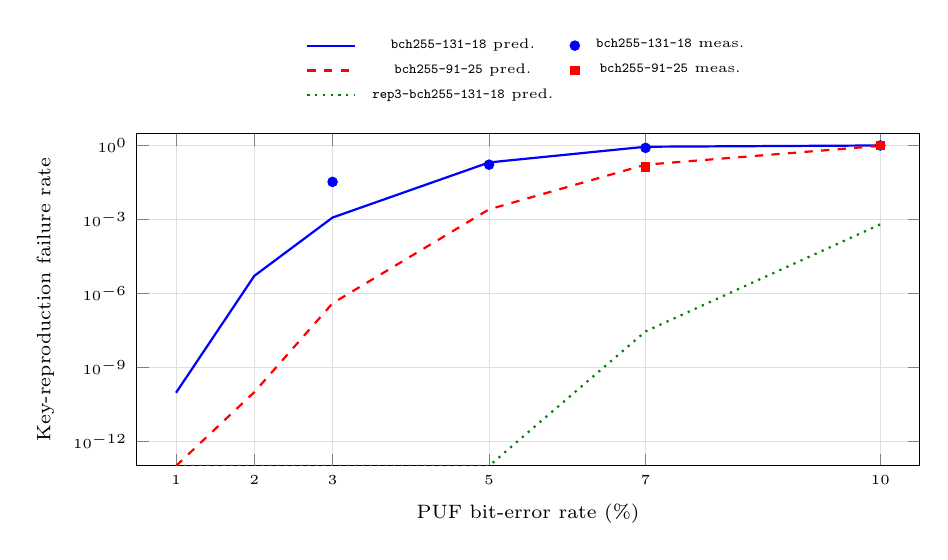
\begin{tikzpicture}
\begin{axis}[
  width=0.95\linewidth, height=5.8cm,
  xlabel={PUF bit-error rate (\%)},
  ylabel={Key-reproduction failure rate},
  xlabel style={font=\scriptsize}, ylabel style={font=\scriptsize},
  ticklabel style={font=\tiny},
  ymode=log, ymin=1e-13, ymax=3, xmin=0.5, xmax=10.5,
  xtick={1,2,3,5,7,10}, ytick={1e-12,1e-9,1e-6,1e-3,1},
  ymajorgrids, xmajorgrids, grid style={gray!25},
  legend style={at={(0.5,1.06)},anchor=south,legend columns=2,font=\tiny,
                draw=none,column sep=4pt},
  ]
\addplot[blue,thick] coordinates
  {(1,9.3e-11) (2,5.12e-6) (3,1.19e-3) (5,2.05e-1) (7,8.89e-1) (10,1.0)};
\addlegendentry{\texttt{bch255-131-18} pred.}
\addplot[only marks,mark=*,mark size=1.7pt,blue] coordinates
  {(3,0.0333) (5,0.1667) (7,0.800) (10,1.000)};
\addlegendentry{\texttt{bch255-131-18} meas.}
\addplot[red,thick,dashed] coordinates
  {(1,1e-13) (2,9.8e-11) (3,3.95e-7) (5,2.56e-3) (7,1.66e-1) (10,9.65e-1)};
\addlegendentry{\texttt{bch255-91-25} pred.}
\addplot[only marks,mark=square*,mark size=1.5pt,red] coordinates
  {(7,0.1333) (10,1.000)};
\addlegendentry{\texttt{bch255-91-25} meas.}
\addplot[green!50!black,thick,dotted] coordinates
  {(1,1e-13) (2,1e-13) (3,1e-13) (5,1e-13) (7,2.86e-8) (10,6.31e-4)};
\addlegendentry{\texttt{rep3-bch255-131-18} pred.}
\end{axis}
\end{tikzpicture}
\caption{Measured key-reproduction failure rate against the analytic binomial
prediction (Table~\ref{tab:noise}). Measured points at exactly zero are omitted
since a log axis cannot represent them; every such point occurs where the
predicted curve is already far below the $1/30$ detection floor, so the
omission hides no disagreement. The concatenated profile measured zero failures
at every tested rate, consistent with its curve remaining orders of magnitude
below the others throughout the swept range.}
\label{fig:rel}
\end{figure}

The default profile reaches a failure rate near $1.2\times10^{-3}$ at 3\%
bit-error rate. A failure probability below $10^{-15}$ is \emph{not} attainable
with a single-layer code at these parameters; the concatenated profile does
reach it, at three times the PUF cost, 3{,}825 against 1{,}020 response bits.
That trade is reported as measured rather than asserted analytically. The
default profile was chosen partly because its failure rate is observable: a
rate of $10^{-15}$ cannot be measured in any feasible Monte Carlo experiment,
so a sweep against it would carry no information.

\subsection{Scalability}
\label{sec:scale}

\begin{figure}[H]
\centering
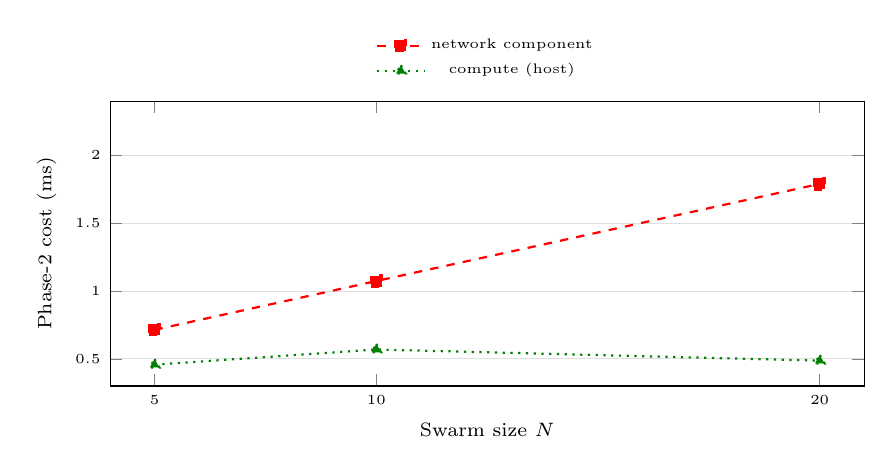
\begin{tikzpicture}
\begin{axis}[
  width=0.92\linewidth, height=5.2cm,
  xlabel={Swarm size $N$}, ylabel={Phase-2 cost (ms)},
  xlabel style={font=\scriptsize}, ylabel style={font=\scriptsize},
  ticklabel style={font=\tiny},
  xmin=4, xmax=21, ymin=0.3, ymax=2.4,
  xtick={5,10,20}, ytick={0.5,1.0,1.5,2.0},
  ymajorgrids, grid style={gray!25},
  legend style={at={(0.5,1.04)},anchor=south,legend columns=1,font=\tiny,
                draw=none},
  ]
\addplot[red,thick,mark=square*,dashed] coordinates {(5,0.7142) (10,1.0737) (20,1.7899)};
\addlegendentry{network component}
\addplot[green!50!black,thick,mark=triangle*,dotted] coordinates {(5,0.4575) (10,0.5693) (20,0.4870)};
\addlegendentry{compute (host)}
\end{axis}
\end{tikzpicture}
\caption{Phase-2 cost against swarm size. The network component grows because
the $M_4$ credential package carries one credential per peer; the per-device
compute stays flat, and per-pair Phase-3 cost was measured independent of $N$
($0.4159$ to $0.4171$~ms across $N=5,10,20$).}
\label{fig:scale}
\end{figure}

Phase 2 is $O(N)$ in swarm size and fully parallel across drones, since each
handshake with the GS is independent. Phase 3 is $O(N^2)$ in total, full-mesh
authentication runs $N(N-1)/2$ exchanges, but constant per pair, as
Section~\ref{sec:eval} measured, and the exchanges are mutually independent; a
deployment that only needs neighbours may authenticate a subset. No per-message
cost grows with the swarm, and the measured growth in Phase-2 elapsed time
(Fig.~\ref{fig:scale}) is a network effect, the growing credential package,
not a compute one.

\subsection{Executed attacks}
\label{sec:attacks}

The theorems of Section~\ref{sec:security} are complemented by executing
attacks against the running protocol. Each configuration declares the outcome
it expects, and the run records whether that expectation held.

A negative control is essential to this argument. Reporting that every attack
failed is unfalsifiable on its own, because it is equally consistent with a
defective adversary. The evaluation therefore includes an \emph{ablation}: a
variant in which one mechanism, the verification of the ground station's
authenticator on $M_2$, is disabled, with everything else unchanged, and the
\emph{same} attacker implementation is run against it. The ablation is a
measurement instrument, not a deployment option; it exists to establish that
the adversary detects a success when one is available.

\begin{table}[H]
\centering
\caption{Attack outcomes, five independent repetitions per attack (eight
attempts per repetition for GS impersonation, one for $M_1$ replay, ten for
credential sniffing). \emph{Oracle} counts UAV responses to forged ground-station
messages. The last row is the ablation in which the verify-before-respond rule
is disabled to validate the adversary}
\label{tab:attacks}
\scriptsize
\setlength{\tabcolsep}{2.4pt}
\begin{tabular}{@{}llccccc@{}}
\toprule
\textbf{Attack} & \textbf{Configuration} & \textbf{Att.} & \textbf{Acc.} &
\textbf{Oracle} & \textbf{Expected} & \textbf{Match} \\
\midrule
GS impersonation & full protocol & 40 & 0 & 0 & fail & yes \\
$M_1$ replay & full protocol & 5 & 0 & 0 & fail & yes \\
Credential sniffing & full protocol & 50 & 0 & 0 & fail & yes \\
\midrule
GS impersonation & \emph{ablation: no P3} & 40 & 5 & 5 & \emph{succeed} & yes \\
\bottomrule
\end{tabular}
\end{table}

Every outcome matches its declared expectation across all five repetitions.
Under the full protocol, forty forged ground-station messages, eight per
repetition times five repetitions, produced no response of any kind: the drone
verifies the authenticator before performing any PUF-dependent computation, so
no challenge--response pair is exposed and the modelling attack of
Corollary~\ref{cor:oracle} has no input to work from. Removing that single
check in the ablation causes the same attacker code to elicit a response and
obtain a challenge--response pair in every one of the five repetitions, which
establishes two things: the adversary detects a success when one exists, so the
zeros above are evidence rather than an artefact, and the verify-before-respond
rule, not some incidental property of the implementation, is what closes the
oracle. Verbatim replay of $M_1$ inside the freshness window is refused by the
nonce cache; the timestamp window alone would admit it. Passive inspection of
$M_4$ across fifty deliveries recovered no per-pair credential, the package
being protected by authenticated encryption.

At the protocol level, capture of one UAV exposes only credentials incident to
that node. In a four-drone configuration this is three of six pairs, against
all six under a swarm-wide credential.

\subsection{UAV mobility}

\subsection{Real 802.11 contention, Phase 3, and mobility}
\label{sec:inet}

Section~\ref{sec:impl-sim} disclosed that the primary link-delay model does not
itself simulate MAC-layer contention, so its network delay is a lower bound. To
bracket that bound with a measured upper one, the same handshake, identical
protocol code, identical crypto suites, identical PUF models, was also driven
over a real IEEE~802.11 ad-hoc stack, the INET framework's
\texttt{Ieee80211ScalarRadioMedium}, with genuine CSMA/CA contention, backoff,
and retransmission. This track covers Phase~2 and Phase~3. No attack results are
claimed here: the passive/active adversary model of Section~\ref{sec:attacks}
depends on a single relay point intercepting every message, which has no
equivalent in a real channel topology where hosts communicate directly.

The single-clock property of this track is what makes a compute/network split
possible here, where it is not on the idealised medium: everything runs on the
simulation clock, so end-to-end wall time genuinely contains the protocol's own
computation, and network is then derived as wall minus compute rather than
measured independently.

\begin{table}[H]
\centering
\caption{Over a real 802.11 stack, thirty runs each. Compute is measured by the
protocol's own timers; Network is \emph{derived} as wall minus compute on this
track's single clock. Motion uses INET's own mobility models}
\label{tab:inet}
\scriptsize
\setlength{\tabcolsep}{2.0pt}
\begin{tabular}{@{}lccccc@{}}
\toprule
\textbf{Configuration} & \textbf{Wall (ms)} & \textbf{Compute} &
\textbf{Network} & \textbf{Ph.\,2} & \textbf{Ph.\,3} \\
 & & \textbf{(ms)} & \textbf{(ms)} & & \\
\midrule
\texttt{Inet80211SHA3} (static) & $11.872{\pm}0.341$ & 0.417 & 11.455 & 300/300 & 2700/2700 \\
\texttt{InetMobLinear}          & $12.141{\pm}0.398$ & 0.425 & 11.716 & 299/300 & 2682/2691 \\
\texttt{InetMobRandom}          & $11.891{\pm}0.391$ & 0.408 & 11.483 & 299/300 & 2682/2685 \\
\midrule
Idealised (Tab.\ \ref{tab:latency}) & --- & 0.569 & 1.074 & 300/300 & 2700/2700 \\
\bottomrule
\end{tabular}
\end{table}

Real CSMA/CA contention costs approximately $7.9\times$ the idealised medium's
network delay for the identical handshake, the genuine price of MAC-layer
realism that the primary model, by construction, cannot show. The compute column
is the useful counterpoint: $0.417$~ms here against $0.569$~ms on the idealised
track, the difference being event-loop overhead the idealised figure still
includes. \textbf{The protocol's own cost does not change when the radio does.}
A tenfold increase in handshake latency is the channel, not the protocol, which
a single combined number would have hidden.

Phase~3 also runs on this track, over the same UDP and 802.11 stack: all 45
pairs of the ten-drone swarm complete, $2700$ of $2700$ peer views under static
positions. Peer authentication therefore does not depend on the idealised
transport for its feasibility. Messages $P_2$ and $P_3$ carry no identity field
on the wire, so the receiving peer names its sender from the datagram's source
port, each drone binding its own; the in-process transport had supplied that
identity for free and INET does not, and recovering it from the L3 address fails
silently because a host holds several addresses and the routed source is not the
one the resolver returns.

Mobility is measured here rather than on the idealised medium, and the reason
governs how the result should be read. On the idealised medium the only quantity
motion changes is propagation delay, nanoseconds over a $500\times300$~m field;
a handshake completes in under $2$~ms of simulated time, during which a drone at
8~m/s covers about $1.2$~cm. A measurement there would be a null result by
construction. On a real stack, received power, SNIR, and hence CSMA/CA
behaviour all depend on live distance, so motion changes the channel
observably. Two configurations use INET's own mobility models
(\texttt{LinearMobility}, \texttt{RandomWaypointMobility}) at 8~m/s: linear
motion costs $12.141{\pm}0.398$~ms against $11.872{\pm}0.341$~ms static, a real
but small $0.27$~ms, and random-waypoint motion at $11.891{\pm}0.391$~ms is
statistically indistinguishable from static. Both complete 299 of 300 Phase-2
handshakes.

The honest summary is that one handshake is short enough relative to the field
that motion barely perturbs it, and the useful contribution of this experiment
is that it holds on a real MAC as well, where the channel is genuinely
distance-dependent. Motion's cumulative effect across many re-authentications as
a drone patrols far from the ground station remains open, and would need a
periodic re-authentication loop rather than the one-shot handshake both tracks
run.

Across the three configurations two Phase-2 handshakes of 900 did not complete.
Both show zero bytes sent and a ground-station attempt count one short of the
full ten, meaning the drone's own fuzzy-extractor reproduction failed before it
ever transmitted $M_1$, the same failure class already reported for
\texttt{ArbiterPuf} and \texttt{HighNoise} in Section~\ref{sec:eval-fun}, not a
new mode introduced by the 802.11 stack. Both drones use the same idealised PUF
model and 3\% bit-error rate as \texttt{StadiumSHA3}, which observed zero such
failures in 300 devices; two failures in a further 900 independent draws of the
same low-probability event is consistent with ordinary sampling variance, not a
rate change.

\subsection{Energy cost}

No energy or power figures should be invented where none were found, and none
here multiply host x86 timing by an embedded power draw, since that product
would have no physical meaning. Every energy figure is either a literature
constant applied as-is (labelled \texttt{estimate:lit}) or that same constant
applied to this work's own measured byte counts (labelled
\texttt{measured-derived}). Table~\ref{tab:energy} lists the constants and names
their provenance, distinguishing what this project measured from what it took
from the literature.

\begin{table}[H]
\centering
\caption{Literature-sourced energy costs. \emph{Verified} means a primary
source's own table was read directly; \emph{unverified} means only a
search-summarised description of a real, findable paper was available}
\label{tab:energy}
\scriptsize
\setlength{\tabcolsep}{2pt}
\begin{tabular}{@{}p{3.2cm}cp{3.85cm}@{}}
\toprule
\textbf{Primitive} & \textbf{Energy} & \textbf{Platform (confidence)} \\
\midrule
SHA3-256 (Keccak-$f[1600]$) & 275~nJ/call & 130nm ASIC, 1~MHz~\cite{sha3_energy_pessl}; unver.\ \\
SPONGENT-160 (serial) & 112.8~nJ/call & 0.13$\mu$m ASIC, 100~kHz~\cite{spongent_original}; ver. \\
SPONGENT-160 (parallel) & 4.02~nJ/call & 0.13$\mu$m ASIC, 100~kHz~\cite{spongent_original}; ver. \\
Ascon-128a & $<$0.75~$\mu$J/byte & nRF5340~\cite{ascon_energy_sorescu}; unver. \\
X25519 scalar mult.\ & 5.14~mJ/call & STM32L152RE~\cite{x25519_energy_franck}; ver. \\
802.11 radio, TX & 50.0~nJ/bit & 802.11a, 6~Mbps~\cite{radio_energy_ergen}; ver. \\
802.11 radio, RX & 30.8~nJ/bit & 802.11a, 6~Mbps~\cite{radio_energy_ergen}; ver. \\
\bottomrule
\end{tabular}
\end{table}

Table~\ref{tab:energy} deliberately omits MAC, KDF, and Extract rows: no
published energy figure was found for these composed constructions, only for
the base hash or permutation each is built on, and this work does not fabricate
a number where none was found. The 802.11 radio figures match this work's own
configured link bitrate of 6~Mbps exactly, so no rate-mismatch caveat is needed
when combining them with measured message sizes.

Combining the X25519 figure with the structural fact that Phase 2 performs one
key generation and one derivation per side per handshake gives $2 \times 5.14
= 10.28$~mJ of ephemeral-exchange energy per side per handshake, for either
suite. Combining the radio figures with this work's measured $M_1$ to $M_4$
byte counts gives $214.0~\mu$J of radio energy for one drone's Phase-2 handshake
under \texttt{StadiumSHA3} ($215.0~\mu$J under \texttt{StadiumSPONGENT},
$147.5~\mu$J at $N=5$, $347.1~\mu$J at $N=20$). Compute therefore dominates the
energy budget by roughly $48\times$ over radio for this handshake: the
ephemeral Diffie--Hellman exchange that buys forward secrecy is the expensive
part of the energy budget, not the symmetric primitives and not the network,
consistent with the latency finding that the mandatory ephemeral exchange, not
the hash/MAC/KDF/AEAD core, is where this protocol pays its price relative to a
scheme without forward secrecy.

%=============================================================================
\section{Discussion}
\label{sec:discussion}
%=============================================================================

\subsection{Scalability}

Phase 2 is $O(N)$ and fully parallel across drones. Phase 3 is $O(N^2)$ in
total but the measurements show a per-pair cost flat across swarm size, and a
deployment that only needs neighbours may authenticate a subset of pairs.
Because every operation is symmetric, a hash, a MAC, an AEAD, a KDF, and one
ephemeral exchange, per-message cost is small and does not grow with the swarm.

\subsection{Design choices}

Three choices give the framework its character. Deriving a \emph{stable} key
from the PUF means the drone stores no secret and can re-authenticate any
number of times from a single enrollment, rather than consuming a limited pool
of challenge--response pairs. Rooting Phase 3 in \emph{per-pair} credentials
rather than one swarm-wide secret means a captured node endangers only its own
links, matching the capture threat that motivates PUFs in the first place.
Making the ephemeral exchange \emph{mandatory} rather than optional means
forward secrecy is a property of every session, not a feature that can be
silently skipped.

\subsection{Noise tolerance}

The BCH(255,131,18) fuzzy extractor corrects up to 18 bit-flips against $7.65$
expected flips in a 255-bit block at a 3\% error rate. That margin is real but
finite, and Section~\ref{sec:reliability} measures where it ends: the default
profile fails to reproduce $\text{mk}_i$ for about one device in a thousand at
3\%, roughly one in six at 5\%, and almost always at 10\%. Three consequences
deserve statement. First, a failure probability below $10^{-15}$ is not
attainable with a single-layer code at these parameters; the concatenated
profile reaches it at three times the PUF cost, and that is the trade rather
than a property of the default configuration. Second, because a block must
exceed the $n-k = 124$ bits the sketch discloses, blocks are 255 bits; a
128-bit block would leak almost all of itself and contribute essentially
nothing to the budget of Eq.~\eqref{eq:budget}. Third, a device that cannot
reproduce its key does not authenticate incorrectly, it does not authenticate
at all, and never transmits a first message. Availability, not security, is
what degrades with environmental noise, and a deployment must budget for
re-enrollment or a stronger profile accordingly.

\subsection{Limitations and future work}

The analysis is at the protocol level. A mechanised end-to-end proof discharged
in the prover, and a hardware prototype on real PUF silicon, are the natural
next steps, as is an empirical study of PUF reliability across environmental
extremes. Dynamic swarm membership, drones joining and leaving during flight,
is left for future work; mobility itself is measured in
Section~\ref{sec:eval}. The full-protocol latency comparison against RSA and
ECDSA is measured in Section~\ref{sec:baseline}, rather than left at the
primitive level, and the contention-aware MAC layer is measured in
Section~\ref{sec:inet}, so the two simplifications of the primary model are now
bracketed by measurements rather than hidden.

%=============================================================================
\section{Conclusion}
\label{sec:concl}
%=============================================================================

This paper presented a four-phase PUF-based authentication framework for UAV
swarms. Its root of trust is a stable key distilled from each drone's own
silicon by a BCH(255,131,18) fuzzy extractor, so no secret is ever stored on
the device. Every handshake message is protected by a keyed MAC, and the raw
PUF response never leaves the drone, which closes the challenge-harvesting
avenue open to designs that transmit the response or a function of it. Peer
authentication runs directly between drones on per-pair credentials delivered
under authenticated encryption during the UAV--GS handshake, so a captured node
compromises only its own links. Every session key folds in a mandatory,
authenticated ephemeral Diffie--Hellman secret, giving perfect forward secrecy.
Six theorems, mutual authentication in both directions, peer authentication,
replay and man-in-the-middle resistance, session-key secrecy, forward secrecy,
and capture boundedness, reduce these properties to standard assumptions and
are mirrored by a Tamarin symbolic model. Built from a 160-bit hash, a keyed
MAC, a lightweight AEAD, a KDF, and one elliptic curve, the framework fits the
resource budget of aerial platforms.

The reference implementation on OMNeT++~6.3 supports the claims with
measurement. All 600 UAVs and all 11{,}400 peer pairs of a twenty-drone swarm
authenticate, at $0.57 \pm 0.04$~ms of compute and $1.07$~ms of modelled
network delay per UAV--GS handshake and $0.4167 \pm 0.0006$~ms per peer pair
over thirty independent
repetitions. The fuzzy extractor's measured failure rate tracks its binomial
prediction across four orders of magnitude, which is the evidence that error
correction genuinely occurs. Executed attacks reproduce the analysis, and an
ablation with the ground-station check removed shows the adversary detects
success when it exists, so the negative results are falsifiable. A real 802.11
stack brackets the idealised-medium latency at $7.9\times$ and carries Phase~3
as well, and there the protocol's own compute is unchanged at $0.42$~ms, so the
increase is the channel rather than the protocol.

Two findings temper the performance narrative and are reported as measured.
Same-platform benchmarks place RSA-2048 verification at $17~\mu$s, so
millisecond-scale figures for that operation, and speedup multipliers derived
from them, are unsound, and this framework's own mandatory ephemeral exchange
costs about as much as a bare ECDH exchange, not an order of magnitude less,
which is the disclosed cost of forward secrecy at the primitive level. At full
protocol scale, measured against real signature-authenticated baselines on the
same simulator, the framework is $2.1\times$ slower than an
ECDSA-authenticated handshake, $1.64$ against $0.79$~ms, the cost of storing no
long-term secret on the device against a scheme whose signing key must be
stored somewhere, while against RSA it comes out narrowly ahead, $1.64$ against
$1.77$~ms, because RSA's own signing cost exceeds this framework's entire
protocol compute. The advantages of the framework are therefore argued as properties
rather than raw speed: no long-term secret on the device, no certificate
infrastructure, peer authentication without a ground-station round trip,
capture damage bounded to a node's own links, and a symmetric core small enough
to leave the hardware-area argument intact.

\begin{thebibliography}{00}

\bibitem{securing_uav_fanet}
A.~Mukherjee, S.~Bose, A.~Mukherjee, and S.~Saha, ``Securing UAV flying ad hoc wireless networks: Authentication development for robust communications,'' \emph{IEEE Access}, vol.~12, pp.~1--15, 2024.

\bibitem{puf_lightweight_uav}
P.~Gope and B.~Sikdar, ``A PUF-based lightweight authentication and key agreement protocol for smart UAV networks,'' \emph{IET Commun.}, vol.~16, no.~18, pp.~2136--2148, 2022.

\bibitem{peer2peer_auth}
T.~Bera, S.~Das, and A.~K.~Das, ``Secure and efficient peer-to-peer authentication-attestation protocol for UAV networks,'' in \emph{Proc. IEEE INFOCOM Workshops}, 2023, pp.~1--6.

\bibitem{puf_ntu}
Nanyang Technological University, ``PUF-based lightweight security framework for drone networks,'' DR-NTU Tech. Rep. Series, 2023.

\bibitem{bch_puf_extraction}
J.~Delvaux, D.~Gu, I.~Verbauwhede, M.~Hiller, and M.-D.~Yu, ``Cryptographic key generation from PUF data using efficient fuzzy extractors,'' \emph{IEEE Trans. Inf. Forensics Security}, vol.~15, pp.~2025--2038, 2020.

\bibitem{sram_puf_bch}
L.~Zhang, Y.~Li, Z.~Wang, and C.~Chen, ``SRAM-PUF key extraction method and performance analysis based on RS and BCH codes,'' \emph{Electronics}, vol.~12, no.~4, p.~1012, 2023.

\bibitem{helper_data_masking}
R.~Maes, ``Helper data masking for physically unclonable function-based key generation,'' \emph{Cryptology ePrint Archive}, Rep. 2019/688, 2019.

\bibitem{puf_iot_strong_adversary}
U.~Chatterjee, R.~S.~Chakraborty, and D.~Mukhopadhyay, ``PUF-based authentication in IoT against strong physical adversary,'' in \emph{Proc. IEEE DATE}, 2022, pp.~1--6.

\bibitem{puf_uav_cross_domain}
B.~Li, H.~Zhu, J.~Shen, and T.~Li, ``PUF-based secure and efficient anonymous authentication protocol for UAV towards cross-domain environments,'' \emph{IEEE Trans. Veh. Technol.}, vol.~72, no.~9, pp.~12101--12115, 2023.

\bibitem{puf_overview}
A.~Alkatheiri, Y.~G.~Alghamdi, and S.~U.~Jan, ``Review of physically unclonable functions (PUFs): Structures, models, and algorithms,'' \emph{Front. Electron.}, vol.~4, 2023.

\bibitem{puf_key_exchange}
R.~Aman, K.~Z.~Ghafoor, and S.~K.~Sood, ``PUF based lightweight authentication and key exchange protocol for IoT,'' in \emph{Proc. IEEE GLOBECOM}, 2022, pp.~1--6.

\bibitem{puf_6g_uav}
S.~Khan, A.~Irshad, S.~A.~Chaudhry, and M.~Alazab, ``A provably secure and lightweight PUF-based authentication scheme for 6G-enabled UAV networks,'' \emph{IEEE Internet Things J.}, vol.~11, no.~5, pp.~8532--8543, 2024.

\bibitem{arbiter_puf_iot}
L.~Xu, X.~Wang, Q.~Li, and H.~Wang, ``An enhanced event-based dynamic authentication protocol leveraging arbiter PUF for IoT devices,'' \emph{IEEE Internet Things J.}, vol.~10, no.~18, pp.~16123--16135, 2023.

\bibitem{lightweight_crypto_evaluation}
T.~Eisenbarth \emph{et al.}, ``Design and evaluation of lightweight cryptographic primitives for constrained devices,'' \emph{J. Cryptographic Eng.}, vol.~12, no.~3, pp.~245--260, 2022.

\bibitem{spongent_original}
A.~Bogdanov, M.~Kne\v{z}evi\'c, G.~Leander, D.~Toz, K.~Var{\i}c{\i}, and I.~Verbauwhede, ``SPONGENT: A lightweight hash function,'' in \emph{Proc. CHES}, LNCS 6917, 2011, pp.~312--325.

\bibitem{sha3_energy_pessl}
P.~Pessl and M.~Hutter, ``Pushing the limits of SHA-3 hardware implementations to fit on RFID,'' in \emph{Proc. CHES}, LNCS 8086, 2013, pp.~126--141.

\bibitem{ascon_energy_sorescu}
A.-M.~Sorescu \emph{et al.}, ``Comparative performance analysis of lightweight cryptographic algorithms on resource-constrained IoT platforms,'' \emph{Sensors}, vol.~25, no.~18, art.~5887, 2025.

\bibitem{x25519_energy_franck}
C.~Franck, J.~Gro{\ss}sch\"adl, Q.~Le~Corre, and C.~Lenou~Tago, ``Energy-scalable Montgomery-curve ECDH key exchange for ARM Cortex-M3 microcontrollers,'' in \emph{Proc. EMSICC}, 2018.

\bibitem{radio_energy_ergen}
M.~Ergen and P.~Varaiya, ``Decomposition of energy consumption in IEEE 802.11,'' Univ.\ California Berkeley EECS, Tech. Rep.

\bibitem{sha3_standard}
NIST, ``SHA-3 standard: Permutation-based hash and extendable-output functions,'' FIPS PUB 202, 2015.

\bibitem{keccak_team}
G.~Bertoni, J.~Daemen, M.~Peeters, and G.~Van~Assche, ``The Keccak reference,'' Version 3.0, 2011.

\bibitem{dolev_yao}
D.~Dolev and A.~Yao, ``On the security of public key protocols,'' \emph{IEEE Trans. Inf. Theory}, vol.~29, no.~2, pp.~198--208, 1983.

\bibitem{dodis_fuzzy}
Y.~Dodis, R.~Ostrovsky, L.~Reyzin, and A.~Smith, ``Fuzzy extractors: How to generate strong keys from biometrics and other noisy data,'' \emph{SIAM J. Comput.}, vol.~38, no.~1, pp.~97--139, 2008.

\bibitem{hkdf}
H.~Krawczyk, ``Cryptographic extraction and key derivation: The HKDF scheme,'' in \emph{Advances in Cryptology --- CRYPTO}, 2010, pp.~631--648.

\bibitem{curve25519}
D.~J.~Bernstein, ``Curve25519: New Diffie--Hellman speed records,'' in \emph{Public Key Cryptography --- PKC}, 2006, pp.~207--228.

\bibitem{ascon}
C.~Dobraunig, M.~Eichlseder, F.~Mendel, and M.~Schl\"affer, ``Ascon v1.2: Lightweight authenticated encryption and hashing,'' \emph{J. Cryptology}, vol.~34, no.~3, 2021.

\bibitem{bellare_rogaway}
M.~Bellare and P.~Rogaway, ``Entity authentication and key distribution,'' in \emph{Advances in Cryptology --- CRYPTO}, 1993, pp.~232--249.

\bibitem{tamarin}
S.~Meier, B.~Schmidt, C.~Cremers, and D.~Basin, ``The TAMARIN prover for the symbolic analysis of security protocols,'' in \emph{Proc. CAV}, 2013, pp.~696--701.

\end{thebibliography}

\end{document}
